\chapter{Contact lexical flow inference}
Having established PLFI as an exploratory tool for detecting directional contact in the linguistic history of a region, we now turn towards the second task which we set out to tackle within the lexical flow framework. After a summary of where we stand after Chapter 6, and after an overview of what will be different in this chapter, in Section 7.2 I explain why the contact flow inference problem has the shape of a causal inference problem with hidden common causes. 

In Section 7.3, I explain why the vanilla RFCI algorithm as introduced towards the end of Chapter 3 for causal inference problems of this shape, is difficult to apply on the basis of noisy cognacy overlap data. Section 7.4 describes my most successful attempt to compensate for these weaknesses, which is to define a significance test for v-structure decisions based on a very close connection with the hypergeometric distribution. The resulting variant of the RFCI algorithm is called Contact Lexical Flow Inference (CLFI), and is presented by both pseudocode and an informal description in Section 7.5. 

Section 7.6 evaluates the different CLFI variants resulting from different approaches for skeleton and arrow inference for the contact flow inference task on the same real and synthetic datasets which were already used in the previous chapter. For this purpose, the evaluation metrics have to be adapted to the new problem, and phylum separation is added as a new performance criterion.

An early version of contact flow inference was previously discussed in \cite{dellert2016a}. There, the method was tested on an older version of NorthEuraLex for a language set similar to the current Uralic case study, with promising results which the version presented in this chapter does not significantly improve upon, although it performs better on other case studies.

\section{The contact flow inference task}
To recapitulate the core ideas of lexical flow inference, we systematically compare the cognate overlaps between pairs of languages with other languages in order to find deletable links in a graph which represent paths of lexical transmission. which we need to. After thinning out the graph structure in this way until no further link can be deleted, we know which contacts we minimally need to assume in order to explain the observable overlap patterns. On this structure, we compare the overlap patterns among triples of languages in order to extract hints of directionality, with the goal of assigning a directionality to each link in the lexical flow network.

In phylogenetic lexical flow inference, the common ancestors of observed languages were modeled explicitly by reconstructed data, turning every language into a mixture of lexical material transmitted via one of the incoming arrows, with some noise added due to lexical replacement. Such a phylogenetic lexical flow network can be interpreted as a full theory of how the lexicon of each observable language was shaped by inheritance and contact. Since the method is in principle powerful enough to reconstruct contact between proto-languages, PLFI is a fully general method for evolutionary network inference.

Contact network inference can be seen as a synchronic variant of the same basic idea, with a more modest goal. We still attempt to infer directional contact, but only on the level of living languages, without trying to infer when in the history of each language the transfer in question happened. We are thus on the very common and familiar description level of talking e.g. about \ili{French} loans in \ili{English} instead of Norman French loans into \ili{Middle English}, which would be more exact from a diachronic perspective, and the desired outcome of phylogenetic flow inference.

Given the shape of the contact flow inference problem, it is obvious that if we continue to treat languages as variables, and measure dependencies between languages in terms of cognacy overlap, we are now faced with hidden common causes, namely the proto-languages which were modeled explicitly in phylogenetic lexical flow inference, and now create overlap that is not explainable by directed lateral transmission.

While being conceptually simpler, contact flow inference is clearly a less natural problem than phylogenetic flow inference. Since its results do not contain any temporal component such as earlier proto-languages, the resulting graphs cannot be considered evolutionary networks by any definition. Moreover, in contact networks similarities due to common inheritance will appear in the shape of bidirected links, and will be difficult to distinguish from bidirectional contact, which will make the resulting graphs more difficult to interpret and evaluate.

\section{Advantages and disadvantages of contact flow}
The decisive advantage of contact flow inference in comparison to phylogenetic flow inference is that by removing the need for reconstructed proto-languages in the cognacy overlap data, we will be getting rid of an important source or errors that we have seen re-appear over and over again in the discussion of the case studies in Chapter 6.

Also, the results will be more grounded in an observable truth, as we do not need to put any possibly unrealistic phylogenetic assumptions into the task, and there is no major parameter like the choice of reconstruction method, which previously influenced result quality so much that it would make or break PLFI as an exploratory tool. In contrast, contact flow inference is a much more data-driven process, and it will not be a surprise that it yields comparatively stable results.

Finally, the absence of the proto-languages leads to a smaller problem size for the causal inference methods. This causes significant reductions in runtime, which can in the worst case increase exponentially with the number of languages. Depending on the variant, executing PLFI on the entire NorthEuraLex dataset (107 languages) takes about two to six hours on a single 2 GHz core, whereas the CLFI analysis developed in this chapter never takes more than 20 minutes. Since this difference is bound to become more pronounced with even larger problems, CLFI is clearly a lot more feasible for large-scale exploratory data analysis.

Coming to the disadvantages of CLFI, implementing and tracing the behavior of the algorithm is quite a bit more challenging than it was for PLFI. Since we can no longer assume causal sufficiency, and enter the realm of causal inference with latent confounders. As the reader will remember from Chapter 3, this type of causal inference requires a lot more formal machinery, leaves much more detail choices in an implementation, and comes with a much smaller treasure of practical experience gained from applying it to different problem domains.

\section{Difficulties in applying the RFCI algorithm}
What happens if we simply use the existing standard algorithm for causal inference in the presence of latent confounders, and run the RFCI algorithm presented in Chapter 3 on our cognacy-based conditional independence test? It turns out that the absence of reconstructed additional languages leads to slightly more reliable independence checks, but that, due to the more comprehensive propagation rules, the consequences of a single wrong result in the v-structure tests can be even more severe than what we have seen in the PLFI case studies.

For instance, consider a run of the RFCI algorithm on the Baltic Sea scenario. Among many correct v-structures such as $fin \arrowOA olo \arrowAO rus$ (\ili{Olonets Karelian} having a large inherited overlap with \ili{Finnish}, and some \ili{Russian} loans), the separating set criterion also creates an erroneous v-structure $olo \arrowOA rus \arrowAO lav$, where Russian looks like a mixture of Olonets Karelian (the Russian loans) and \ili{Latvian} (the inherited stock of shared Balto-Slavic words). Now, the (arguably correct) absence of a different v-structure leads to a first propagation, turning $olo \arrowAA rus \arrowOO pol$ into $olo \arrowAA rus \arrowLA pol$. $rus \arrowLA pol$ is an acceptable arrow (there are indeed some Russian loans in \ili{Polish}, in addition to the common Slavic material inherited by both languages), but this is more of a lucky coincidence. In the next reasoning step, the new arrow into Polish creates one of the preconditions for one of the RFCI-specific propagation patterns, 
namely rule $\mathcal{R}4$. The pattern in question is $rus \arrowAO lit \arrowOA pol \arrowAL rus$, for which the bidirected erroneous arc provides a discriminating path $olo \arrowAA rus \arrowAO lit \arrowOA pol$, on which it turns out impossible to delete any link, which leads to $rus \arrowAA lit \arrowAA pol \arrowAL rus$. Finally, the new bidirected link combines with the non-collider $pol \arrowAA lit \arrowOA lav$ to create the wrong arrow $lit \arrowLA lav$. To summarize, it turns out that the root cause for the erroneous arrow between two \ili{Baltic languages} was a failed v-structure check involving a Uralic minority language in Russia. While the details of these computations might have been difficult to follow, it should have become very clear to how much trouble a single erroneous v-structure test can lead in the RFCI algorithm, and why this means we cannot expect vanilla RFCI to work well on our noisy data. On the plus side, even when the RFCI rules $\mathcal{R}5$ to $\mathcal{R}7$ dealing with selection bias were activated, they were almost never applied in my test runs, showing that at least the absence of selection bias is detected by RFCI.

While my independence tests appear to be good enough for direct application in RFCI, for the v-structure tests I again need to rely on specialized more stable heuristics such as UFR and TSS. In phylogenetic flow inference, every collider had the shape $A \arrowLA B \arrowAL C$, representing the lexicon of $B$ to be a mixture of material from languages $A$ and $B$. The problem in contact flow inference is that colliders can now be formed by any combination of bidirectional and directional arcs. Since bidirectional links represent the existence of hidden common causes, we would expect every link between related languages to be bidirectional, whereras cross-family contacts should lead to unidirectional links. Consequently, we get colliders that represent very different underlying histories.

For the Baltic Sea scenario, the collider $swe \arrowLA fin \arrowAA krl$ arises from a situation where one of two closely related languages borrows material from a language that belongs to a different family. In constrast, the collider $deu \arrowLA ekk \arrowAL rus$ represents two cross-family contacts where the donor languages are related. Each of these different scenarios will lead to radically different three-way overlapping patterns, making collider tests much more difficult. For instance, the first collider will not lead to any overlap between \ili{Swedish} and \ili{Karelian}, whereas such overlap exists for the second collider, due to both donor languages being related.

While it would be conceivable to extend TSS to cover the new problem shape, but instead of fitting the three-way overlap to one possible collider scenario $A \arrowLA B \arrowAL C$, we now have to model four different scenarios, and derive predictions for each of these scenarios in order to catch the full range of overlap patterns which can result from local collider scenarios. This leads to a much more difficult problem shape for the already difficult binary classification problem to decide whether a triple of languages forms a collider or not. Instead of going down this not very promising road, I will now develop an alternative test which does not rely on triangle scores, but still performs better than the separating set criterion.
 
\section{Significance testing for v-structures}
Taking a step back from the RFCI algorithm and considering the problem of inferring v-structures from cognacy data, it turns out that the basic intuition behind the criterion applied by the algorithms can be tested much more strictly on discrete cognacy overlap data. Recall again that the essential idea behind inferring a v-structure $A \rightarrow B \leftarrow C$ in the PC and RFCI algorithms was to decide whether $B$ was necessary to separate $A$ and $C$. What does this mean in terms of overlaps between cognate sets?

The observation I used in deriving UFR was that for $B$ not to be necessary for separation, all cognate sets with reflexes in $A$ and $C$ must also have had reflexes in neighbors forming possible flow paths between $A$ and $C$ not going through $B$. For instance, to show that \ili{English} was not necessary to separate Icelandic from French, and therefore establishing English as a collider in this triangle, we need to show that there is an alternative path by which all the overlap between Icelandic and French can be explained. The problem in contact flow inference is that these alternative flow paths are not necessarily visible any longer, because they could actually involve proto-languages, as is the case between Icelandic and French, which share some lexical material due to their common Indo-European ancestry. Unless we have other Indo-European languages which form possible flow paths, $A$ and $C$ might therefore share some lexical material which cannot be explained by any path through the network except through $B$, but the three languages still form a collider $A \rightarrow B \leftarrow C$.

These considerations give rise to a possibly more robust way of testing unshielded triples for v-structures. The question is how to test that $c(A,B,C)$, the count of cognates shared between all three varieties, is significantly smaller than the number we would expect under any of the other causal scenarios. To predict this number, we assume (as before) that when a language borrows lexical material from another, it will sample the lexical material to borrow from the donor language independently from a different language borrowing from the same donor. While this assumption might not be warranted in every individual case (e.g., the name for a newly introduced trade good will often be introduced to many neighboring languages simultaneously), we can still assume this independence of contacts, because there is no obvious mechanism which would coordinate the shape of linguistic influence between two different pairs of languages across their lexicons. In order to violate the independence assumption, such a mechanism would have to make it more likely for words in $B$ which are already borrowings from $A$ to be borrowed further by $C$ from $B$. On rare occasions, such a preference might occur if e.g. the loans from $A$ fit much better into the phonetic system of $C$, but this would clearly be an exceptional case that will not be frequent enough to warrant the costs of foregoing a generally applicable heuristic.

The direct consequence of this independence assumption is that under any of the three scenarios $A \rightarrow B \rightarrow C$, $A \leftarrow B \rightarrow C$, and $A \leftarrow B \leftarrow C$, the overall ratio of shared cognates should be roughly equal to the product of the ratio of shared cognates on each of the two links. For instance, if \ili{Turkish} borrows 30\% of its vocabulary from \ili{Persian}, and \ili{Albanian} borrows 20\% of its vocabulary from Turkish, we would expect 6\% of the Albanian lexicon to be of Persian origin. Now assume that the actual amount of lexical overlap between Albanian and Persian was determined to be 5\%. How can we decide that the observed ratio $\delta$ (5\%) is significantly different from the $\hat{\delta}$ (6\%) we derived? There is no obvious way to model the distribution of either in a way that would provide a reliable statistical test, and my previous solutions (UFR and TSS directionality inference) both relied on what could be called a local explainability 
assumption. This assumption that the local scenario completely explains the overlap pattern in each triangle was already a problematic assumption before, even though adding some tolerance through threshold values turned out to work well enough. In the presence of latent confounders, however, the local explainability assumption is violated in most triangles, because in very many cases there will be in overlap due to relationship between at least two out of the three languages.

Sticking closer to the discrete nature of lexical flow as we conceive of it, it turns out that under the null hypothesis that some scenario other than $A \rightarrow B \leftarrow C$ holds, $c(A,B,C)$ should follow a hypergeometric distribution. To see this, picture the set $cog(B)$ as an urn containing all the cognate classes with reflexes in the language $B$. Picture some of these classes as colored in red, namely the ones shared with $A$, i.e. all the members of $cog(A,B)$. From this urn, we now randomly pick $c(B,C)$ cognate sets, and ask the question how many of these will be colored red, i.e.\ have reflexes in $A$, to predict the count $c(A,B,C)$ of cognate clases shared by all three languages. This immediately gives us a significance test for v-structures, with p-values directly given by the cumulative distribution function of $Hypergeo(c(B),c(A,B),c(B,C))$ at the true value of $c(A,B,C)$.

As an example, take a triple of \ili{Russian} (\textit{rus}) and two Siberian minority languages which are neither related nor have plausibly been in contact, such as \ili{Itelmen} (\textit{itl}) and \ili{Selkup} (\textit{sel}). The cognacy overlaps derived from NorthEuraLex are $c(rus) = 1037$, $c(itl,rus) = 68$, $c(rus,sel) = 100$, and $c(itl,rus,sel) = 27$. Will we reject the null hypothesis that these three languages form a non-collider, i.e.\ correctly conclude that they do not form a v-structure $itl \arrowOA rus \arrowAO sel$? It turns out that we can with surprisingly high confidence, as $chyper(27, 68, 969, 100) = 0.9999999999984805$, i.e.\ we would not expect to find an overlap pattern like this even if we sampled billions of v-structures. It should be obvious that this is a lot more reliable than building on a separating set criterion.

For an example of a true v-structure, consider another triple of languages consisting of again \ili{Russian} plus \ili{Evenki} (\textit{evn}) and \ili{Manchu} (\textit{mnc}). As determined when discussing the contact languages of Uralic, the true structure here should be $rus \rightarrow evn \leftarrow mnc$. On my automatically inferred cognates, the overlaps are $c(evn) = 1224$, $c(rus,evn) = 66$, $c(evn,mnc) = 134$, and $c(rus,evn,mnc) = 2$. The p-value for the hypergeometric test is $chyper(2, 66, 1158, 134) = 0.01745$, which is below any reasonable significance threshold, allowing us to reject any local causal scenario except the desired v-structure.

In what follows, I will write $vStructTest(A \rightarrow B \leftarrow C)$ for language variables to express a v-structure check. In the FCI directionality inference variant, this will denote the usual check in the first separating set that is found. VCI will be used to denote the variant where it means checking whether $chyper(c(A,B,C),c(A,B),c(B)-c(A,B),c(B,C)) < 0.05$, i.e.\ the v-structure test developed here at a significance level of $0.05$. UFR will continue to be used for the unique correlate flow check as introduced in the previous chapter.

\section{Contact Lexical Flow Inference (CLFI)}
Algorithm \ref{clfi-algorithm} shows the adaptations needed to implement the \isi{Contact Lexical Flow Inference (CLFI)} algorithm. The dependency on a tree and an ancestral state reconstruction method is gone, but the propagation rules have become more numerous. This method can only represent the rough structure of the RFCI methods, the way in which the skeleton is revised during the propagation stage cannot be represented in a compact way. The full details of the method need to be taken from Section 3.2.4, and the literature quoted there.

Like PLFI, the algorithm starts out with a fully connected graph, and attempts to find separating sets of increasing size $s$. In each iteration for a given size of separating sets, all links which still exist are sorted by the strength of the remaining flow, so that the algorithm first tries to remove the weakest links, and proceeds to the stronger ones later. Depending on the skeleton inference method, separating set candidates of size $s$ for the pair of languages connected by the current link are formed either from the remaining neighbours of both nodes, or only from sets of other nodes that form connection paths between the two languages. If a separating set was found, the current link is removed from the graph. Up to this point, the algorithm is thus identical to CLFI, except that no reconstructed proto-languages are added to the dataset, and no predefined links are added based on the guide tree.

The algorithms mainly differ in the second stage, if directionality inference methods other than vanilla PC or TSS are used. As explained in Chapter 3, a successful v-structure test in the FCI algorithm no longer leads to the addition of fully directed arrows $L_i \arrowLA L_j \arrowAL L_k$, but to underspecified arrows $L_i \arrowOA L_j \arrowAO L_k$ that can later become either bidirectional or unidirectional arrows. This happens either through additional successful v-structure tests, or through one of the propagation rules $\mathcal{R}_1$ through $\mathcal{R}_{10}$ as described in Chapter 3. The resulting structure is a contact flow network consisting of both bidirected and directed arcs.

\begin{algorithm}\small
  \begin{algorithmic}[1]
  \STATE skeleton inference method $sklM \in \{PC,FS\}$
  \STATE directionality inference method $dirM \in \{VPC,FCI,VCI,UFR,TSS\}\)
  \STATE $\mathcal{L} := \{L_1,\dots,L_n\}$, only the input languages
  \STATE $G := (\mathcal{L},E) := (\mathcal{L},\{\{L_i,L_j\}\ |\ L_i, L_j \in \mathcal{L'}\})$, the complete graph
  \STATE $S \colon \mathcal{L} \times \mathcal{L} \rightarrow \wp(\mathcal{L})$, the separating set storage
  \STATE $s := 0$
  \WHILE{$s < |\mathcal{L}| - 2$}
    \FOR{$\{L_i,L_j\} \in G$ by increasing strength of remaining flow}
      \IF {$sklM = PC$}
        \FOR{each subset $S \in \wp(N)$ for neighbours $N$ of $L_i$ or $L_j$}
	   \IF {$|S| = s$ and $I(L_i;L_j|S) < 0.025$}
	      \STATE remove $\{L_i,L_j\}$ from $G$, $S(L_i,L_j) := S(L_i,L_j) \cup \{S\}$
	   \ENDIF
	\ENDFOR
      \ELSIF {$sklM = FS$}
	\FOR{each combination $P_1,...,P_k$ of paths from $L_i$ to $L_j$ of length $\leq 4$}
	  \IF {$|S| = s$ for $S := \bigcup\{P_1,\dots,P_k\}$}
	    \IF {ratio of $c(L_i,L_j)$ not explainable by flow across $S$ is $<$ 0.025}
		\STATE remove $\{L_i,L_j\}$ from $G$, $S(L_i,L_j) := S(L_i,L_j) \cup \{S\}$
	    \ENDIF
	  \ENDIF
	\ENDFOR
      \ENDIF
    \ENDFOR
    \STATE $s := s + 1$
  \ENDWHILE
  \IF {$dirM = TSS$}
    \FOR{$\{L_i,L_j\} \in G$}
      \IF{$sc(L_i \arrowLA L_j) < 0.72$}
         \STATE add arrow $L_i \rightarrow L_j$ to network
      \ENDIF
    \ENDFOR
  \ELSE
    \FOR{$L_i,L_j,L_k \in \mathcal{L}$ where $\{L_i,L_j\},\{L_j,L_k\} \in E$ but $\{L_i,L_k\} \notin E$}
      \IF{$(L_i \rightarrow L_j \leftarrow L_k)$ is a v-structure according to $dirM$ and $S(L_i,L_k)$}
	\STATE add arrow $L_i \arrowOA L_j$ to network
	\STATE add arrow $L_k \arrowOA L_j$ to network
      \ENDIF
    \ENDFOR
    \STATE propagate arrows according to $\mathcal{R}_1$ to $\mathcal{R}_3$ (if $dirM = VPC$) or $\mathcal{R}_1$ to $\mathcal{R}_{10}$ 
  \ENDIF
  \RETURN network consisting of $G$ and arrows
  \end{algorithmic}
  \caption{CLFI($L_1,\dots,L_n$)}
  \label{clfi-algorithm}
\end{algorithm}

\section{Evaluation of CLFI}
The structure of this section exactly mirrors the order in which PLFI evaluation was performed in the last chapter. I start by discussing the behavior of the evaluation metrics developed there on the contact flow inference problem, and introducing an additional performance measure which captures how well the phylogenetic units are separated in the result network. Then, I again decide on one CLFI variant for the case studies by means of global results on the entire NorthEuraLex dataset. The discussion of the case studies refers back to the previous discussion of PLFI performance in each case study, and mainly discusses the differences in behaviour, instead of going through each of the problems that persist again. The chapter closes with a validation of the findings about the relative performance of CLFI variants against the simulated data.

\subsection{Evaluation metrics for contact flow}
The results of CLFI can largely be evaluated just like PLFI, given a gold standard graph over the living languages in the dataset. The only difficult question is how a gold standard defined in terms of proto-languages can be flattened into a gold standard on the contact flow level. This ties back to the discussion of the NorthEuraLex gold standard in Chapter 4, where the question was whether we should expect each lexical transfer between proto-languages to be represented as an arrow between one pair of descendant languages in the result.

For contact flow inference, the problem is aggravated by the fact that each such contact can only be visible as an arrow between descendant languages. One could certainly argue that ancient influence of e.g.\ Proto-Iranian on Proto-Uralic will justify any arrow from an Iranian\il{Iranian languages} into a Uralic language\il{Uralic languages}, for instance from \ili{Persian} into \ili{Udmurt}. From the viewpoint of arrow evaluation, such an arrow would be a true positive. The difficult question is whether the absence of such an arrow also constitutes a false negative. From a local perspective, it is clear that intensive contact between proto-languages should lead to an overlap, detectable as caused by contact, between any pair of descendant languages. However, the lexical flow separation criterion implements a version of Occam's razor when it comes to leaving links in the skeleton, typically leaving only one entry point (e.g.\ Udmurt) for the borrowed material, and then using the existing network among 
related languages to distribute the material to the other Uralic languages. From the user's perspective, having a graph that is not cluttered by links between each pair of Uralic and Iranian languages, but still containing the essential information that there was influence of some Iranian on some Uralic language, might be the better solution, especially if the link connects the two languages where the contact is most visible, already indicating a good entry point for closer investigation. Still, relaxing the criterion for false negatives in the skeleton to the point where, say, any influence from some Indo-European on some Uralic language would cover all of the individual contacts we were previously interested in (\ili{Swedish} on \ili{Finnish} vs. \ili{German} on \ili{Estonian}, for instance), is certainly not the way to go for a quantitative evaluation.

Due to the difficulty in finding a good definition of false negatives, I opted for the local perspective, counting many false negatives for contacts between proto-languages that are actually represented in a satisfactory manner. This means that all the numbers for skeleton recall I will be reporting do not reflect the actual quality of the networks, although they still fulfill their primary purpose of being able to compare the performance of CLFI variants.

Finally, there is one additional level on which contact flow networks can be evaluated. Since this time, we are not putting any phylogenetic information into the procedure, we can evaluate the result in terms of how well it captures the phylogenetic signal in the data. Ideally, the contact network should connect all languages that belong to the same phylum by a subnetwork of bidirected edges (reflecting the common proto-language as the hidden common cause), while at the same time, all links across phyla should not involve hidden common causes, and therefore be monodirectional. This implies a separation of phyla by directed arcs, and can be quantified by a \textit{\isi{phylum separation score}}, simply defined as the percentage of pairs of languages where the separation induced by the contact flow network (connection or non-connection by a path of bidirected edges) agrees with the separation defined by language family. The phylum separation score will be used as an additional point of evaluation on the 
simulated data.

\subsection{Overall quantitative results for NorthEuraLex data}
Again, I start by quantitatively evaluating the flow networks produced by different variants of the CLFI algorithm on the entire NorthEuraLex dataset against the gold standard, and we first consider skeleton and arrow performance separately. Table \ref{contact-skeleton-evaluation-nelex} compares the skeleton precision and recall. Remember that due to the way false negatives are counted, the skeleton recall suggests a lot more information loss than is actually readable from the output. While the differences between the different methods are much less pronounced than they were for PLFI, the main trend in these results is clearly in favor of flow separation. In both cases, the RFCI skeleton is identical or almost identical to the PC skeleton, indicating that discriminating paths do not form very often in this application if the checks are performed based on flow separation.

\begin{table}[h]
 \centering
 \begin{tabular}{ccccc}
  \hline \hline
   & \multicolumn{2}{l}{Overlap separation} & \multicolumn{2}{l}{Flow separation}\\ 
   & VPC & FCI & VPC & FCI\\ 
  \hline
  skPrc & \textbf{0.969} & 0.961 & 0.922 & 0.922\\
  skRec & 0.314 & 0.265 & \textbf{0.407} & \textbf{0.407}\\
  skFsc & 0.475 & 0.416 & \textbf{0.565} & \textbf{0.565}\\
  \hline
 \end{tabular}
 \caption{Comparing CLFI variants for contact skeleton performance.}
 \label{contact-skeleton-evaluation-nelex}
\end{table}

As before, arrow performance can only be measured on the intersection of links in the inferred skeleton and the gold standard, which will be a smaller or a larger set depending on the skeleton performance. Therefore, arrow performance cannot be reliably compared across reconstructions and skeleton inference variants. Still, we can compare the performance of the four directionality inference methods on the RFCI skeleton. This is done in Table \ref{contact-arrow-evaluation-nelex}. We see that vanilla FCI performs very poorly on the better skeleton, clearly motivating the use of more advanced collider tests. Interestingly, the hypergeometric test with FCI propagation is outperformed by TSS-based directionality inference on both skeletons, indicating that TSS is a useful general-purpose method that might also be of help in causal inference on other types of noisy data. Finally, the weakness of UFR, its dependence on correctly inferred unshielded triples, becomes a strength on the thinned-out overlap skeleton, 
where it outperforms all other methods, whereas it performs worse than VCI on the more dense flow separation skeleton.

\begin{table}[h]
 \centering
 \begin{tabular}{cccccc}
 \hline \hline
   & \multicolumn{5}{l}{Overlap separation}\\ 
        &   VPC &   FCI &   VCI &   UFR &   TSS\\ 
 \hline
  arPrc & 0.150 & \textbf{0.234} & 0.171 & 0.231 & 0.233\\
  arRec & 0.400 & 0.379 & 0.444 & \textbf{0.512} & 0.400\\
  arFsc & 0.219 & 0.289 & 0.247 & \textbf{0.318} & 0.294\\
  \hline
 \end{tabular}\\[0.5cm]
  \begin{tabular}{cccccc}
 \hline \hline
   & \multicolumn{5}{l}{Flow separation}\\ 
        &   VPC &   FCI &   VCI &   UFR &   TSS\\ 
 \hline
  arPrc & 0.113 & 0.167 & 0.323 & 0.309 & \textbf{0.396}\\
  arRec & 0.138 & 0.145 & \textbf{0.721} & 0.691 & 0.677\\
  arFsc & 0.124 & 0.155 & 0.446 & 0.427 & \textbf{0.500}\\
  \hline
 \end{tabular}
 \caption{Comparing CLFI variants for arrow performance.}
 \label{contact-arrow-evaluation-nelex}
\end{table}

Again, the different variants can be ranked by an overall performance score defined as the product of skeleton and arrow F-scores. The resulting ranking in Table \ref{contact-variant-comparison-nelex}, and the higher arrow precision value for the TSS method, suggest to use the FS-TSS variant for the case studies. Compared to PLFI, the skeleton precision is slightly better in CLFI, although the mentioned problem with the counting of false negatives brings the skeleton F-score into regions lower than the PLFI results. Arrow performance even of the best methods is worse than the values attained for PLFI by some margin, reflecting that the arrow inference task is more difficult without causal sufficiency. As for PLFI, the vanilla variant of the respective standard algorithm (FCI/VPC) does not work well due to the high noise level that needs to be compensated by more robust tests.

\begin{table}[h]
 \centering
 \begin{tabular}{lccc}
 \hline \hline
  CLFI Variant & skFsc & arFsc & skFsc $\ast$ arFsc\\ 
 \hline
\texttt{FS-TSS} & 0.565 & 0.500 & 0.283\\
\texttt{FS-VCI} & 0.565 & 0.446 & 0.252\\
\texttt{FS-UFR} & 0.565 & 0.428 & 0.242\\
\texttt{OS-UFR} & 0.475 & 0.318 & 0.151\\
\texttt{OS-TSS} & 0.475 & 0.294 & 0.140\\
\texttt{OS-FCI} & 0.475 & 0.290 & 0.137\\
\texttt{OS-VPC} & 0.475 & 0.219 & 0.104\\
\texttt{OS-VCI} & 0.416 & 0.247 & 0.103\\
\texttt{FS-FCI} & 0.565 & 0.155 & 0.088\\
\texttt{FS-VPC} & 0.565 & 0.124 & 0.071\\
  \hline
 \end{tabular}
 \caption{CLFI variants ranked by combined F-Score on the NorthEuraLex data.}
 \label{contact-variant-comparison-nelex}
\end{table}

\subsection{Qualitative discussion of NorthEuraLex scenarios}
Getting back to the case studies, this time I use the FS-TSS variant of the CLFI algorithm on the same data, and again visualize the difference to the gold standard in the form of evaluation graphs, with the same color coding as before. Due to the false negative issue, we can expect to see many more dotted arrows in light gray this time, indicating how many links in the skeleton were counted as missing, and explaining in a visual way how the low skeleton recall values came about.

 \subsubsection{Case study 1: the Baltic Sea area}
Repeating othe first experiment on the Baltic Sea data, we see in Figure \ref{baltic-result-contact} that most of the contacts which were inferred successfully by PLFI appear in the contact flow network as well. As discussed in the PLFI case study, the problem with the influence of \ili{German} on \ili{Livonian} disappears under the TSS criterion. However, two other problems have appeared instead.

Firstly, CLFI shares the problem that it is most parsimonious for the model to explain away the influence of $deu$ on $lav$ by conditioning on $liv$,  such that \ili{Livonian} is inferred as acting as an intermediary for the transport of \ili{German} lexical material into \ili{Latvian}. This complements the now correctly detected v-structure pattern $deu \arrowLA liv \arrowAL lav$, and produces an additional arrow $liv \arrowLA lav$ which combines into the erroneous bidirected arrow. Note that \ili{Dutch} as a proxy for \ili{Low German} serves a role here again, this time explaining the West Germanic loans in Latvian that cannot have traveled via Livonian because they are not attested there.

Secondly, in measuring the influences between \ili{Slavic languages}, \ili{Belarusian} is seen as influencing \ili{Polish} instead of either a bidirected arrow representing common descent, or a directed arrow from Polish into Belarusian as according to the gold standard. The very strong score ratio of 2.333 in favor of the wrong direction is mainly due (25.8\% of the weight) to an almost perfect fit of the overlap between the two languages and \ili{Russian} to the v-structure $bel \arrowLA pol \arrowAL rus$. Here again, the abstraction to the level of cognacy overlaps shows its weaknesses, as correctly determining the direction of borrowing between these languages can only be done by looking at the actual word forms, and analysing the sound changes.

 \begin{figure}[h!]
 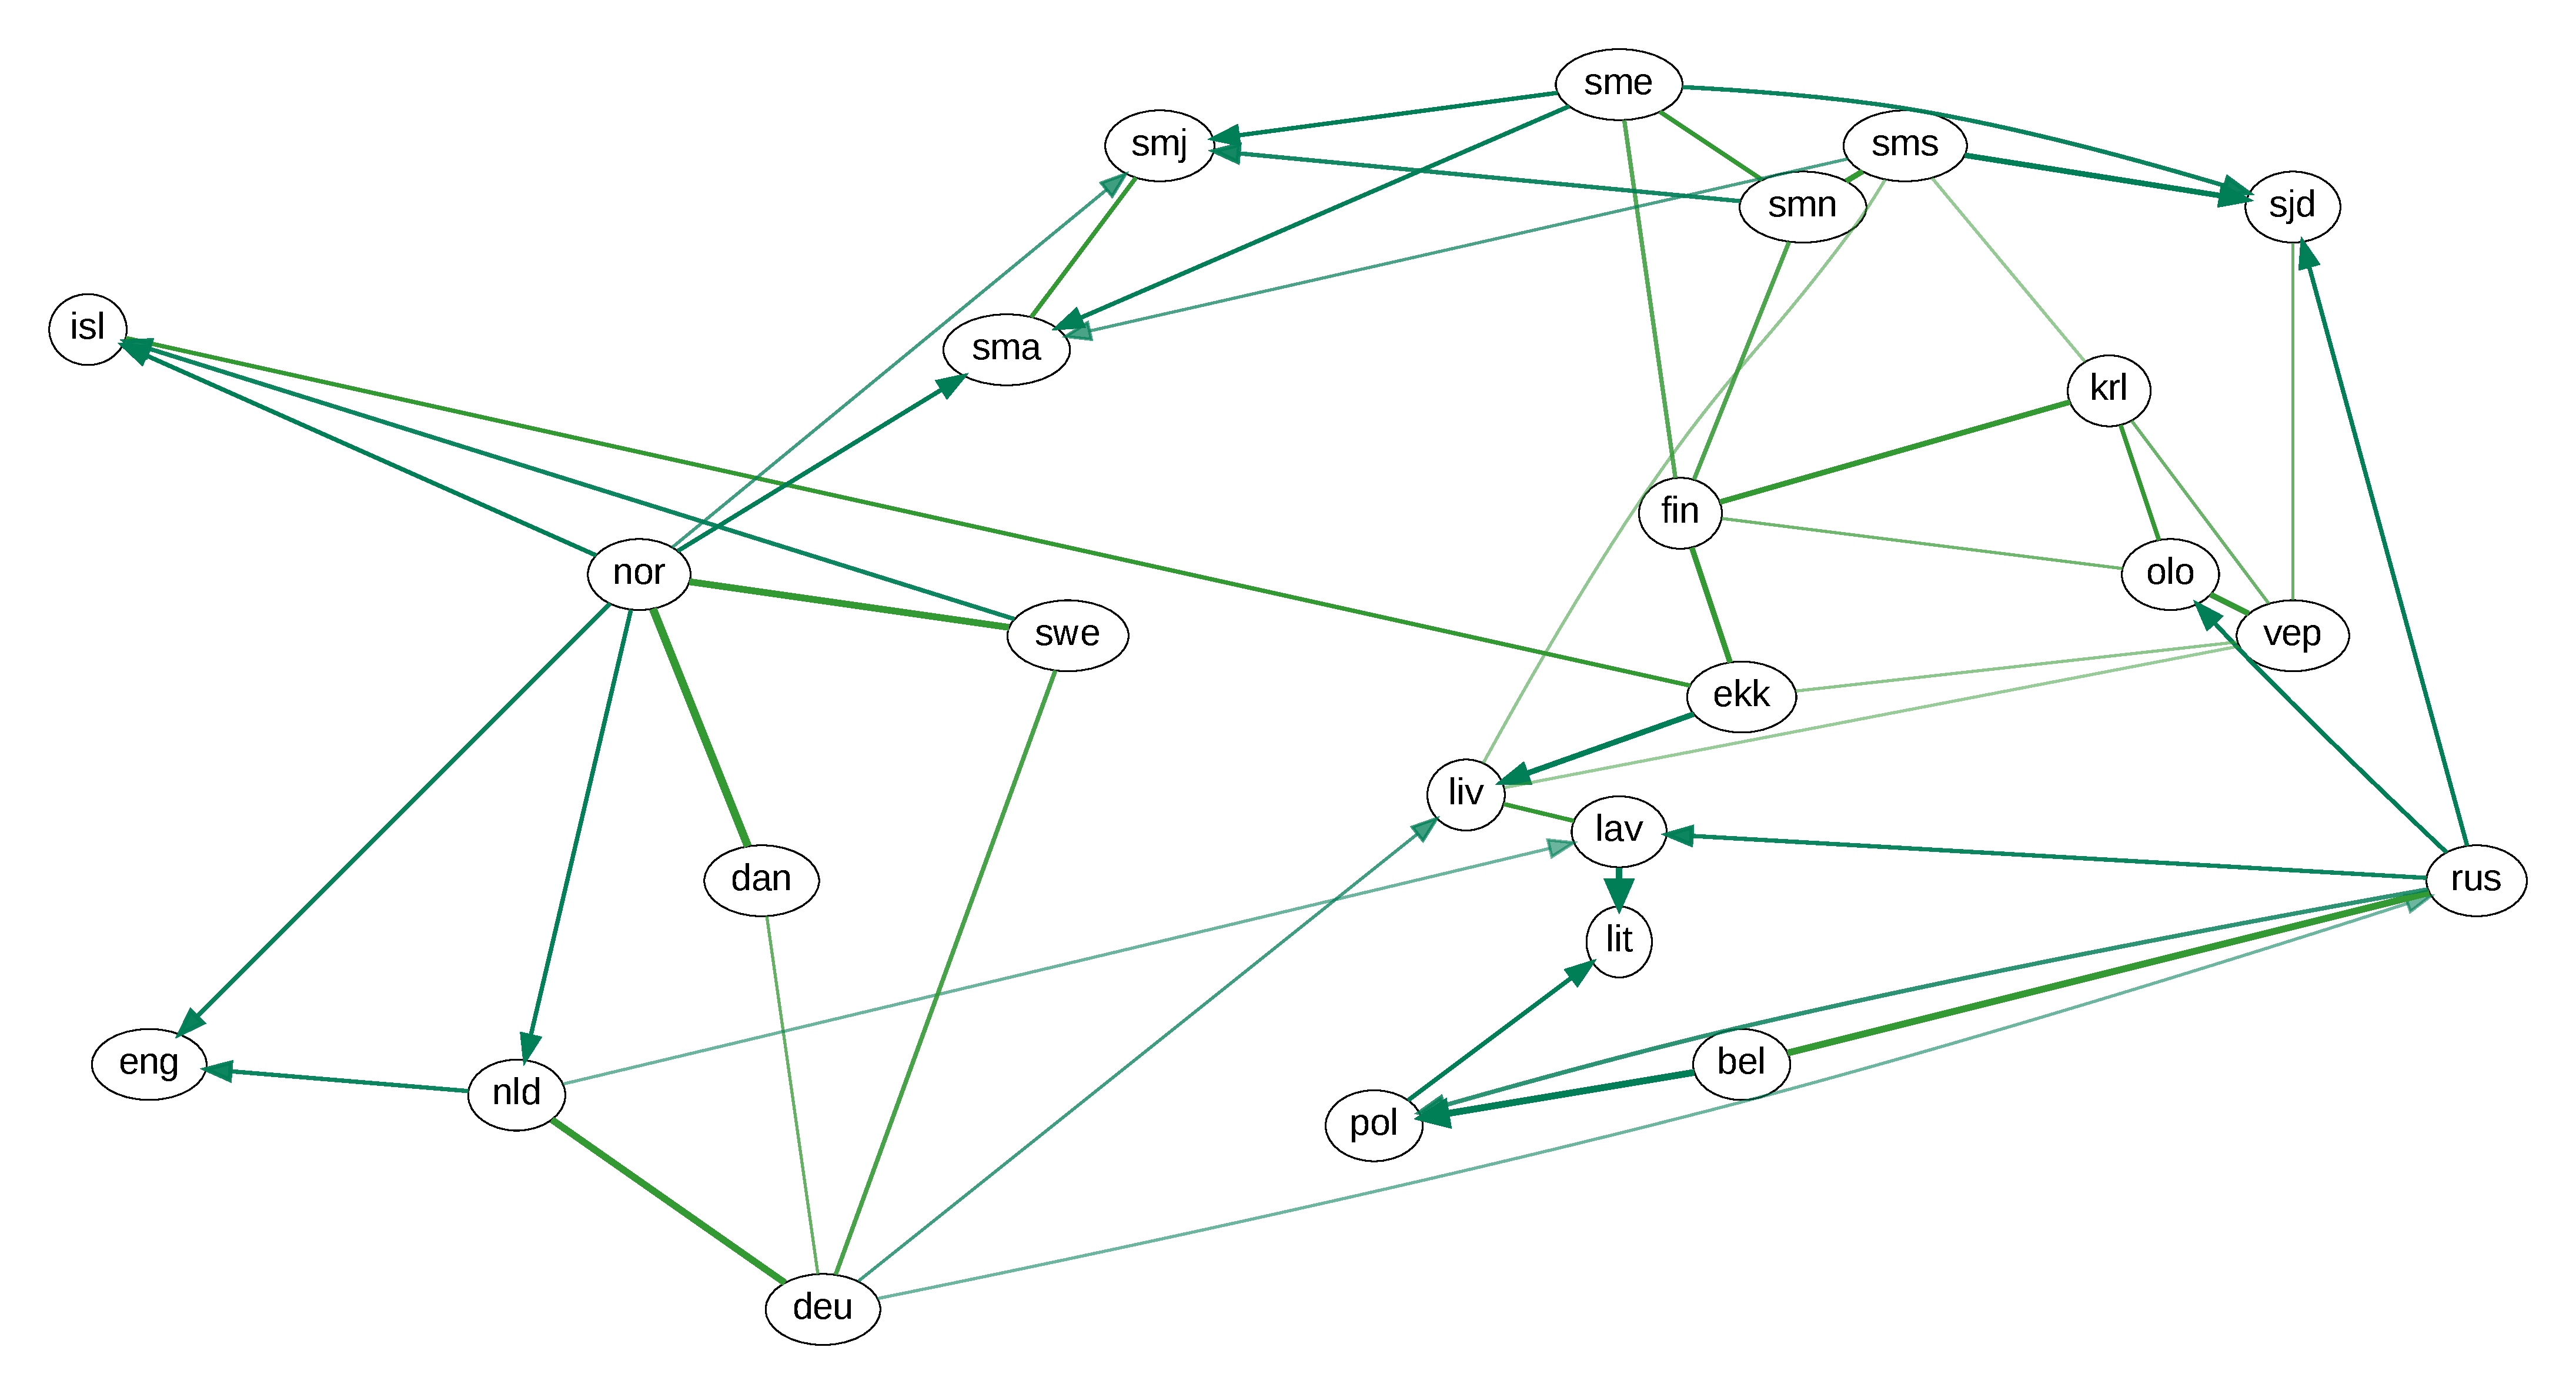
\includegraphics[width=\textwidth]{figures/baltic-contact-fs-tss.pdf}
 \vspace*{5mm}
 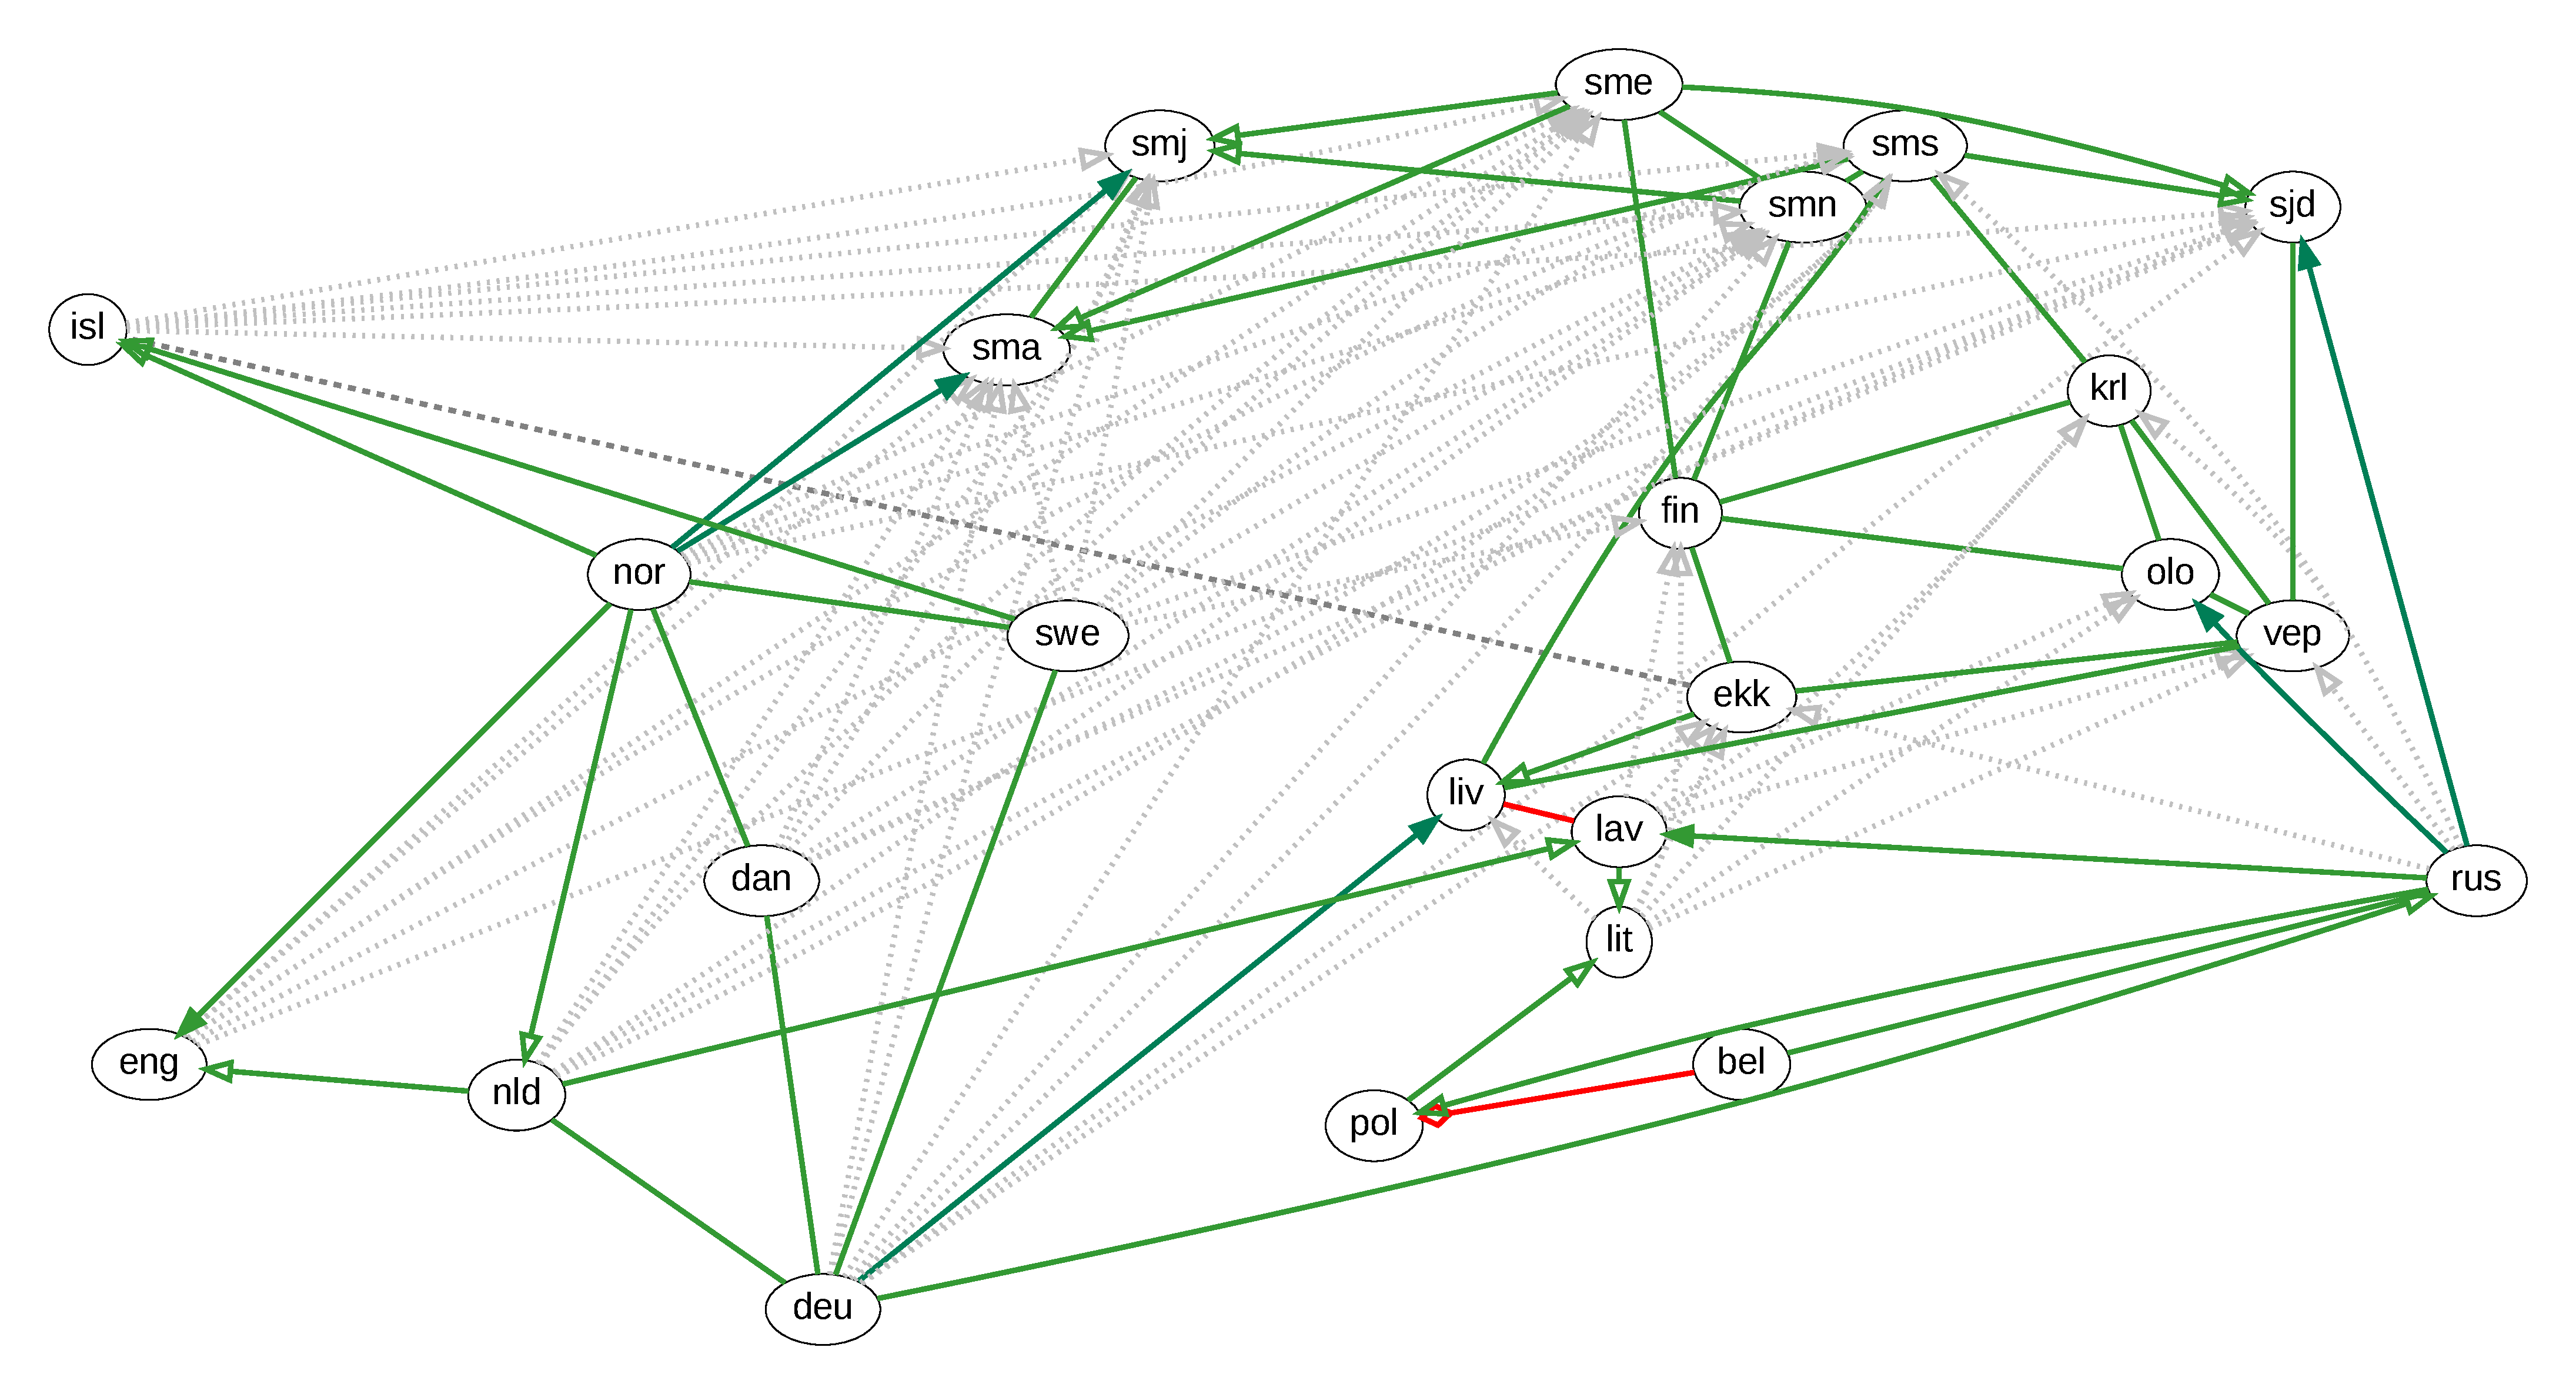
\includegraphics[width=\textwidth]{figures/baltic-contact-fs-tss-eval.pdf}
 \caption{Result and evaluation of contact flow on Baltic Sea data.}
 \label{baltic-result-contact}
 \end{figure}
 
 \subsubsection{Case study 2: Uralic and contact languages}
 \begin{figure}[h!]
 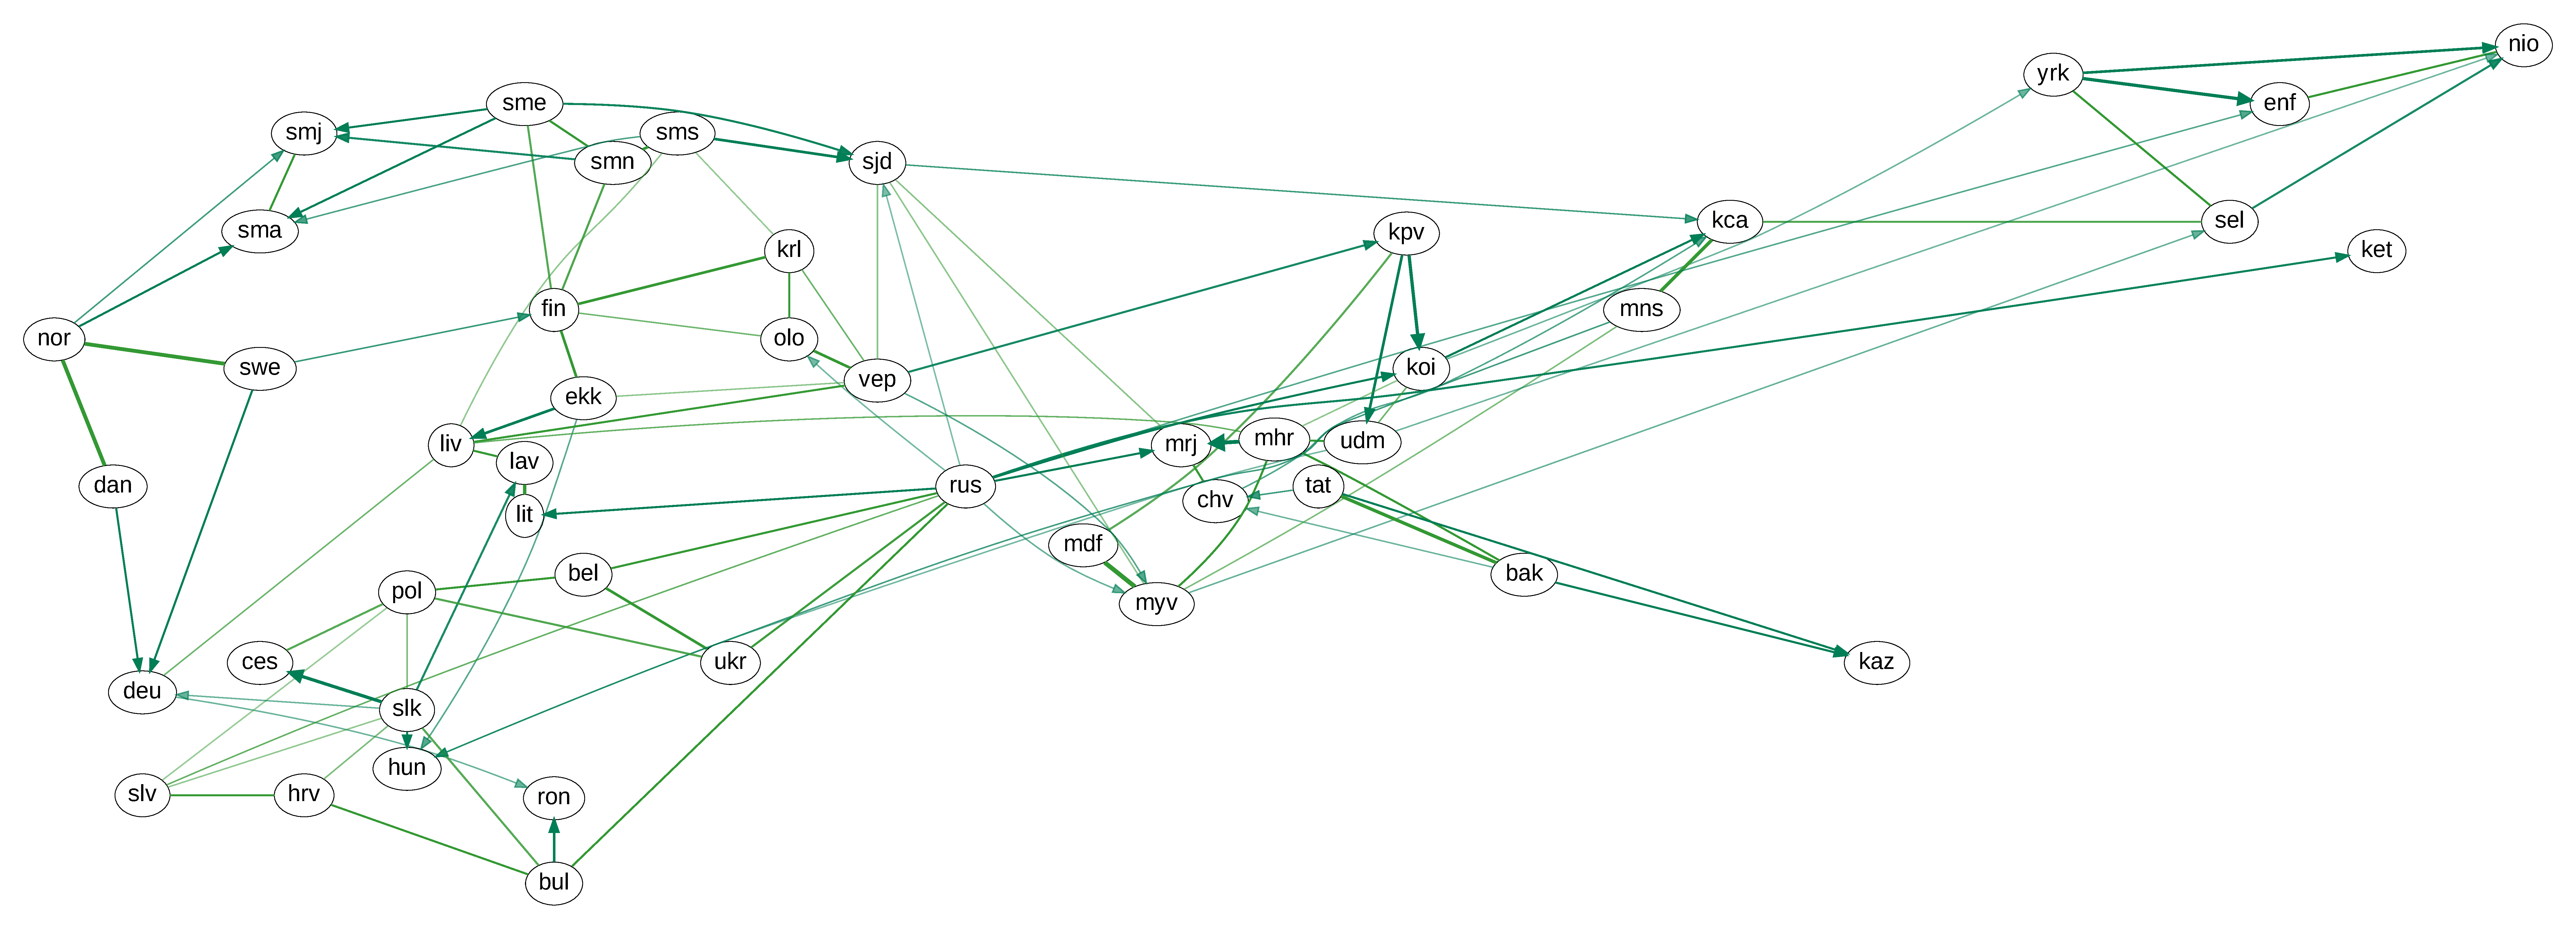
\includegraphics[width=\textwidth]{figures/uralic-contact-fs-tss.pdf}
 \vspace*{5mm}
 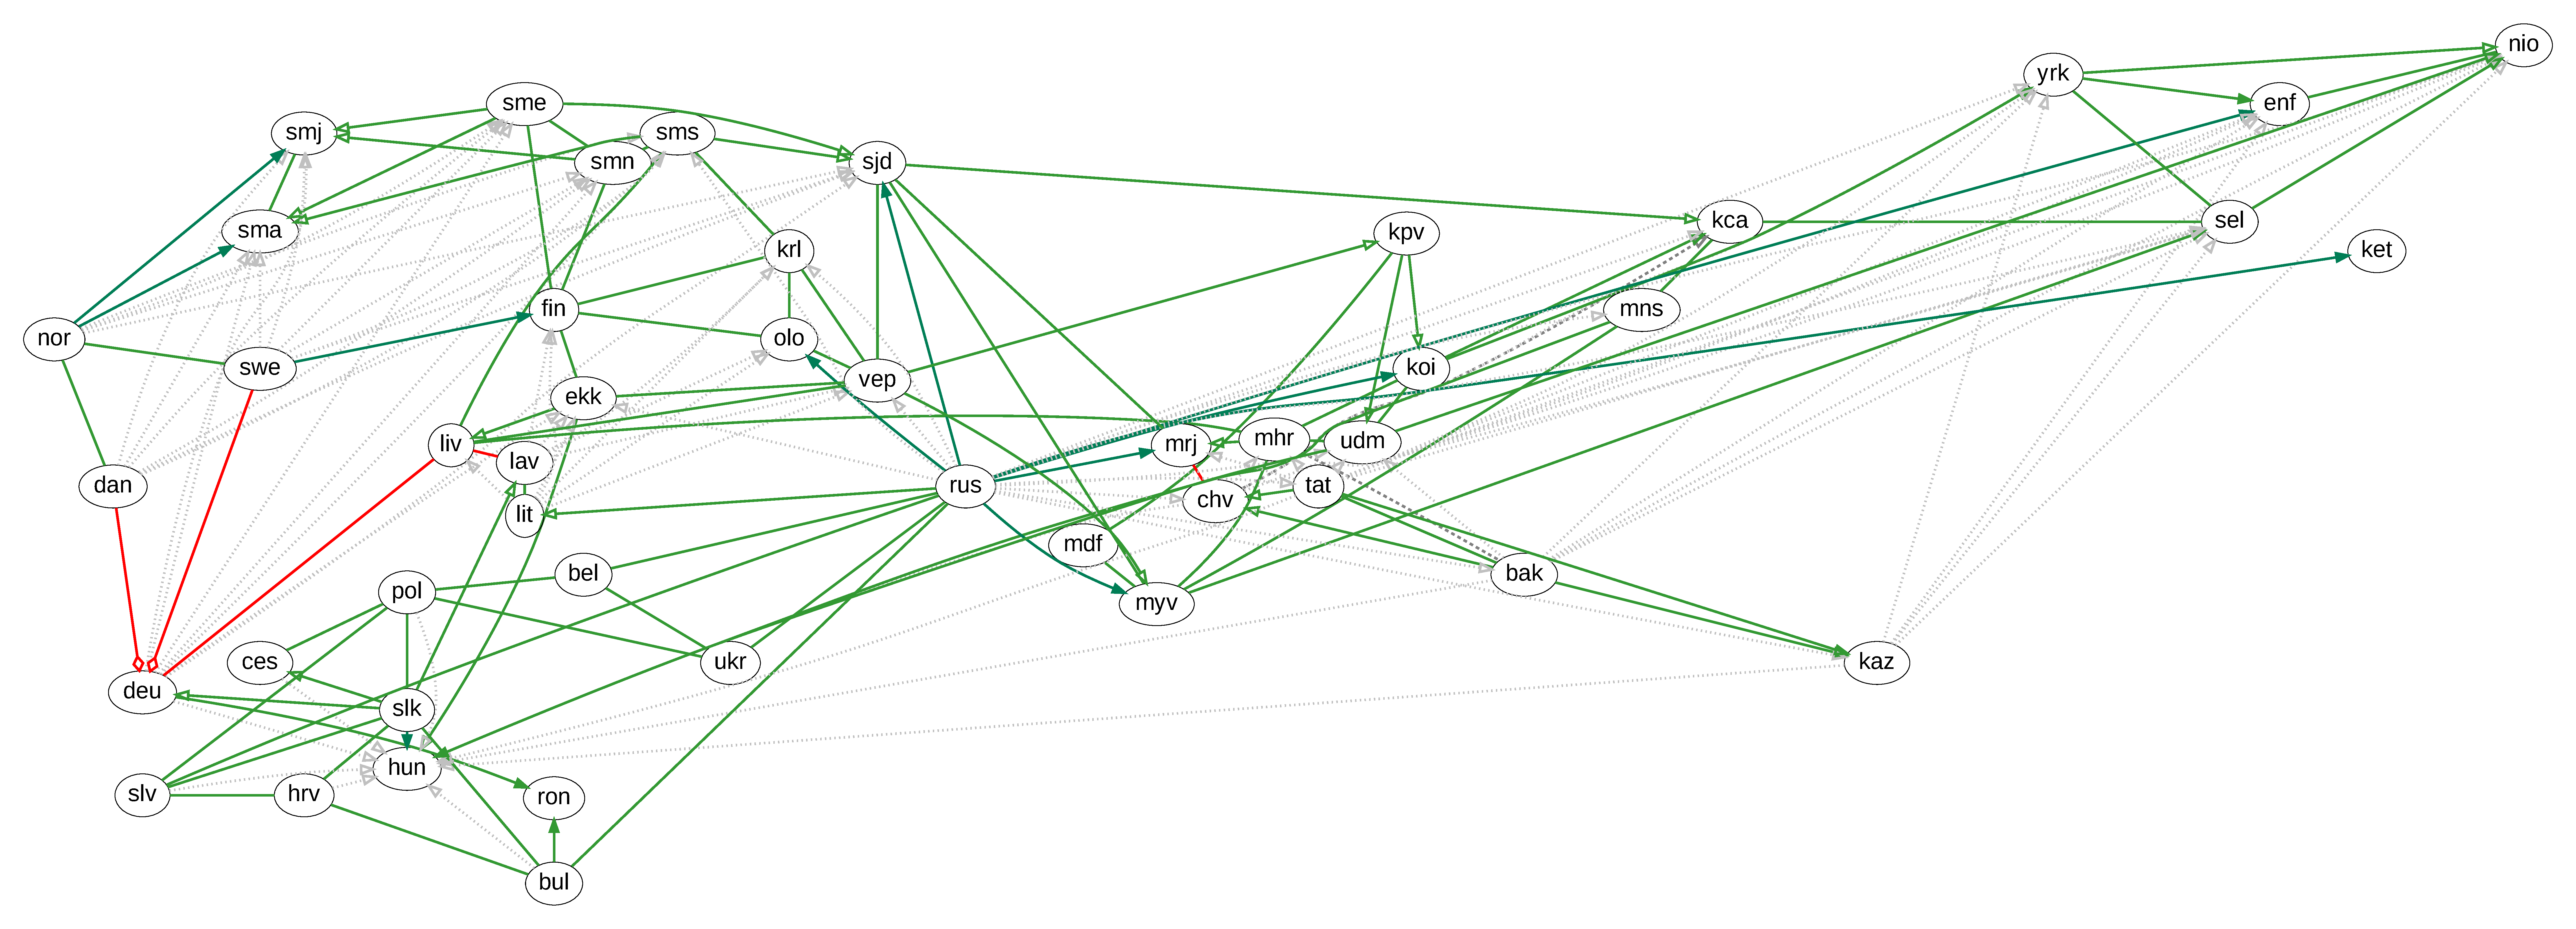
\includegraphics[width=\textwidth]{figures/uralic-contact-fs-tss-eval.pdf}
 \caption{Result and evaluation of contact flow on Uralic data.}
 \label{uralic-result-contact}
 \end{figure}
 
The overall results on the Uralic case study, visualized in Figure \ref{uralic-result-contact}, are again quite convincing, especially in terms of phyla separation, with the exception of \ili{Kazakh} ($kaz$), which becomes separated from the other \ili{Turkic languages} by erroneous incoming directed arcs, and the wrong bidirected link between Latvian and Livonian that were already explained in the first case study.
 
The only major problem with this result is a very interesting cluster of inverted arrows into \ili{German}, which did not appear in the smaller Baltic scenario, although it included all the involved languages as well. For \ili{Danish} and German, the triangles with \ili{Swedish} and \ili{Norwegian} are the only two relevant ones, and the same holds for Norwegian and Danish in reversed roles. The problem now is that all triples fit the v-structure assumption very well. For instance, for $dan \arrowLL deu \arrowLL nor$ we have a predicted overlap of 471 cognates according to the formula I derived, at an observed overlap of 482. The counterevidence scores for all triangles are below 0.1, i.e. they all fit the v-structure assumption very well. The problem is that the scenarios with German at the center tend to fit the v-structure assumption slightly better, so that we have a small amount of evidence against $deu \arrowLA dan$. The TSS score definition only builds on the ratio of scores, not on the actual 
strength of evidence, which leads to a TSS score ratio of 1.8 in favour of $dan \arrowLA deu$. On the Baltic sea scenario, this did not happen because \ili{Dutch} and \ili{English} provided further sources of high-overlap triples counterbalancing this difference. In general, having more languages in the dataset will always increase the stability of TSS, because there are more weighty triples to factor in. The fewer high-weight triangles are available for a language pair, the more unstable the TSS decision will be. We are going to see this effect very strongly in the Siberian case study.

Apart from this cluster of inverted arrows, the inferred contact flow network does not have any serious problems. The empty green arrows in the evaluation graph might serve to highlight a general difficulty of contact flow inference, however. To explain why so much spurious family-internal directionality is inferred, let us consider the \ili{Saami languages}. Like the other \ili{Western Saami languages}, \ili{Northern Saami} ($sme$) has loans from \ili{Norwegian}, but virtually all of these also exist in the smaller Saami languages that have been in even closer contact with Scandinavian languages. This means that it is most parsimonious for the model to explain away the connection from $sme$ to $nor$ by conditioning on $sma$ and $smj$. Locally, this causes the two languages to look like mixtures of their more easterly relatives with Norwegian, leading to directional arrows from $sme$ and $smn$ into $sma$ and $smj$.

\subsubsection{Case study 3: the linguistic landscape of Siberia}
 
\begin{figure}[ht!]
 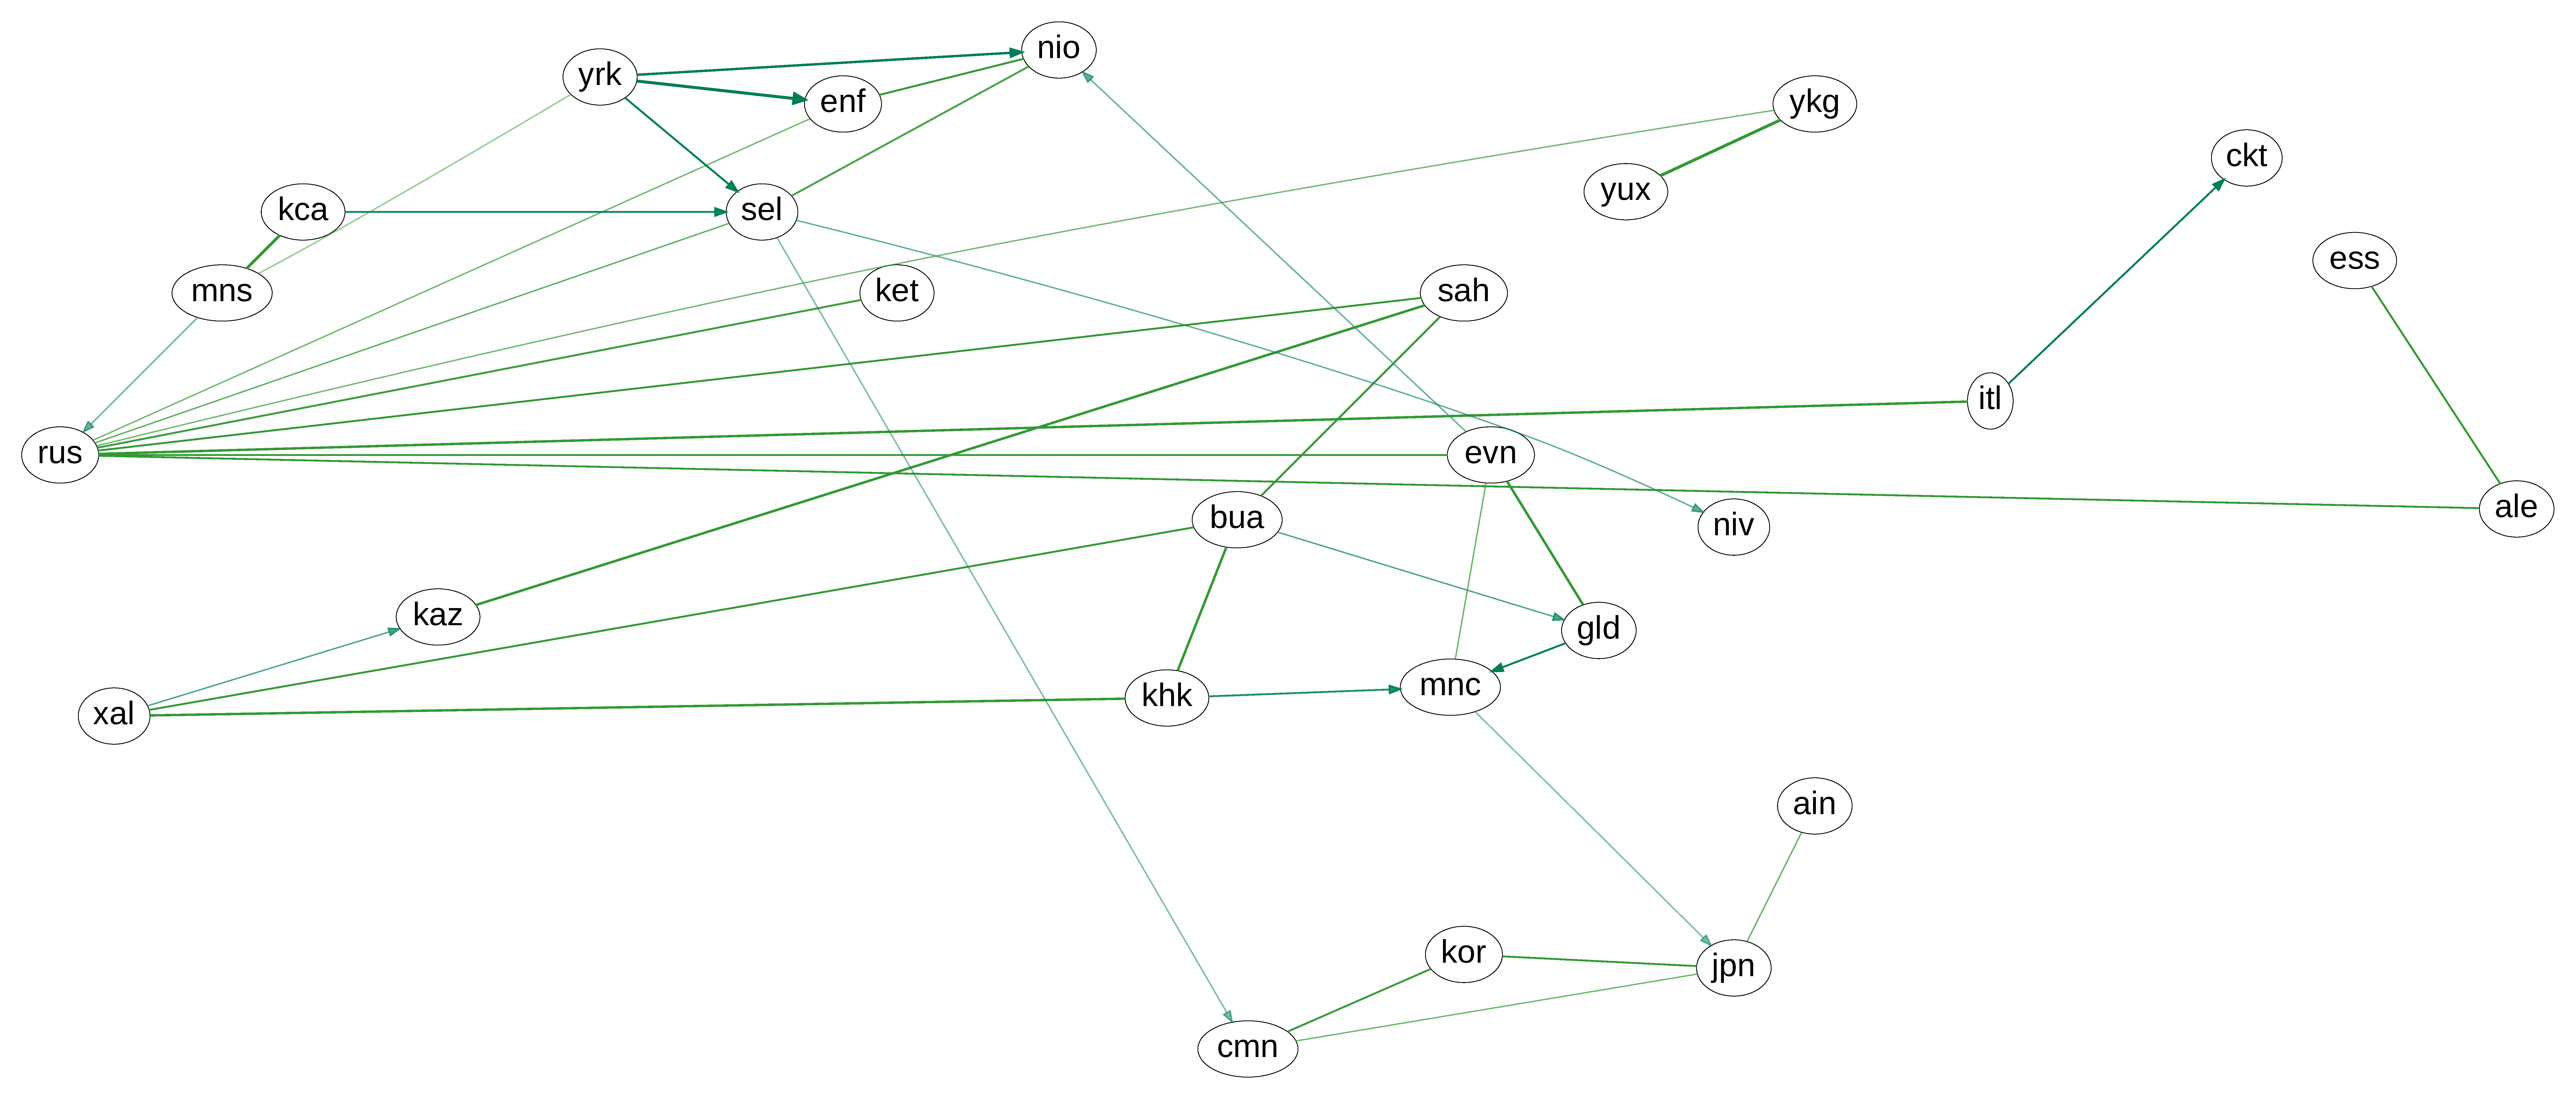
\includegraphics[width=\textwidth]{figures/siberia-contact-fs-tss.pdf}
 \vspace*{5mm}
 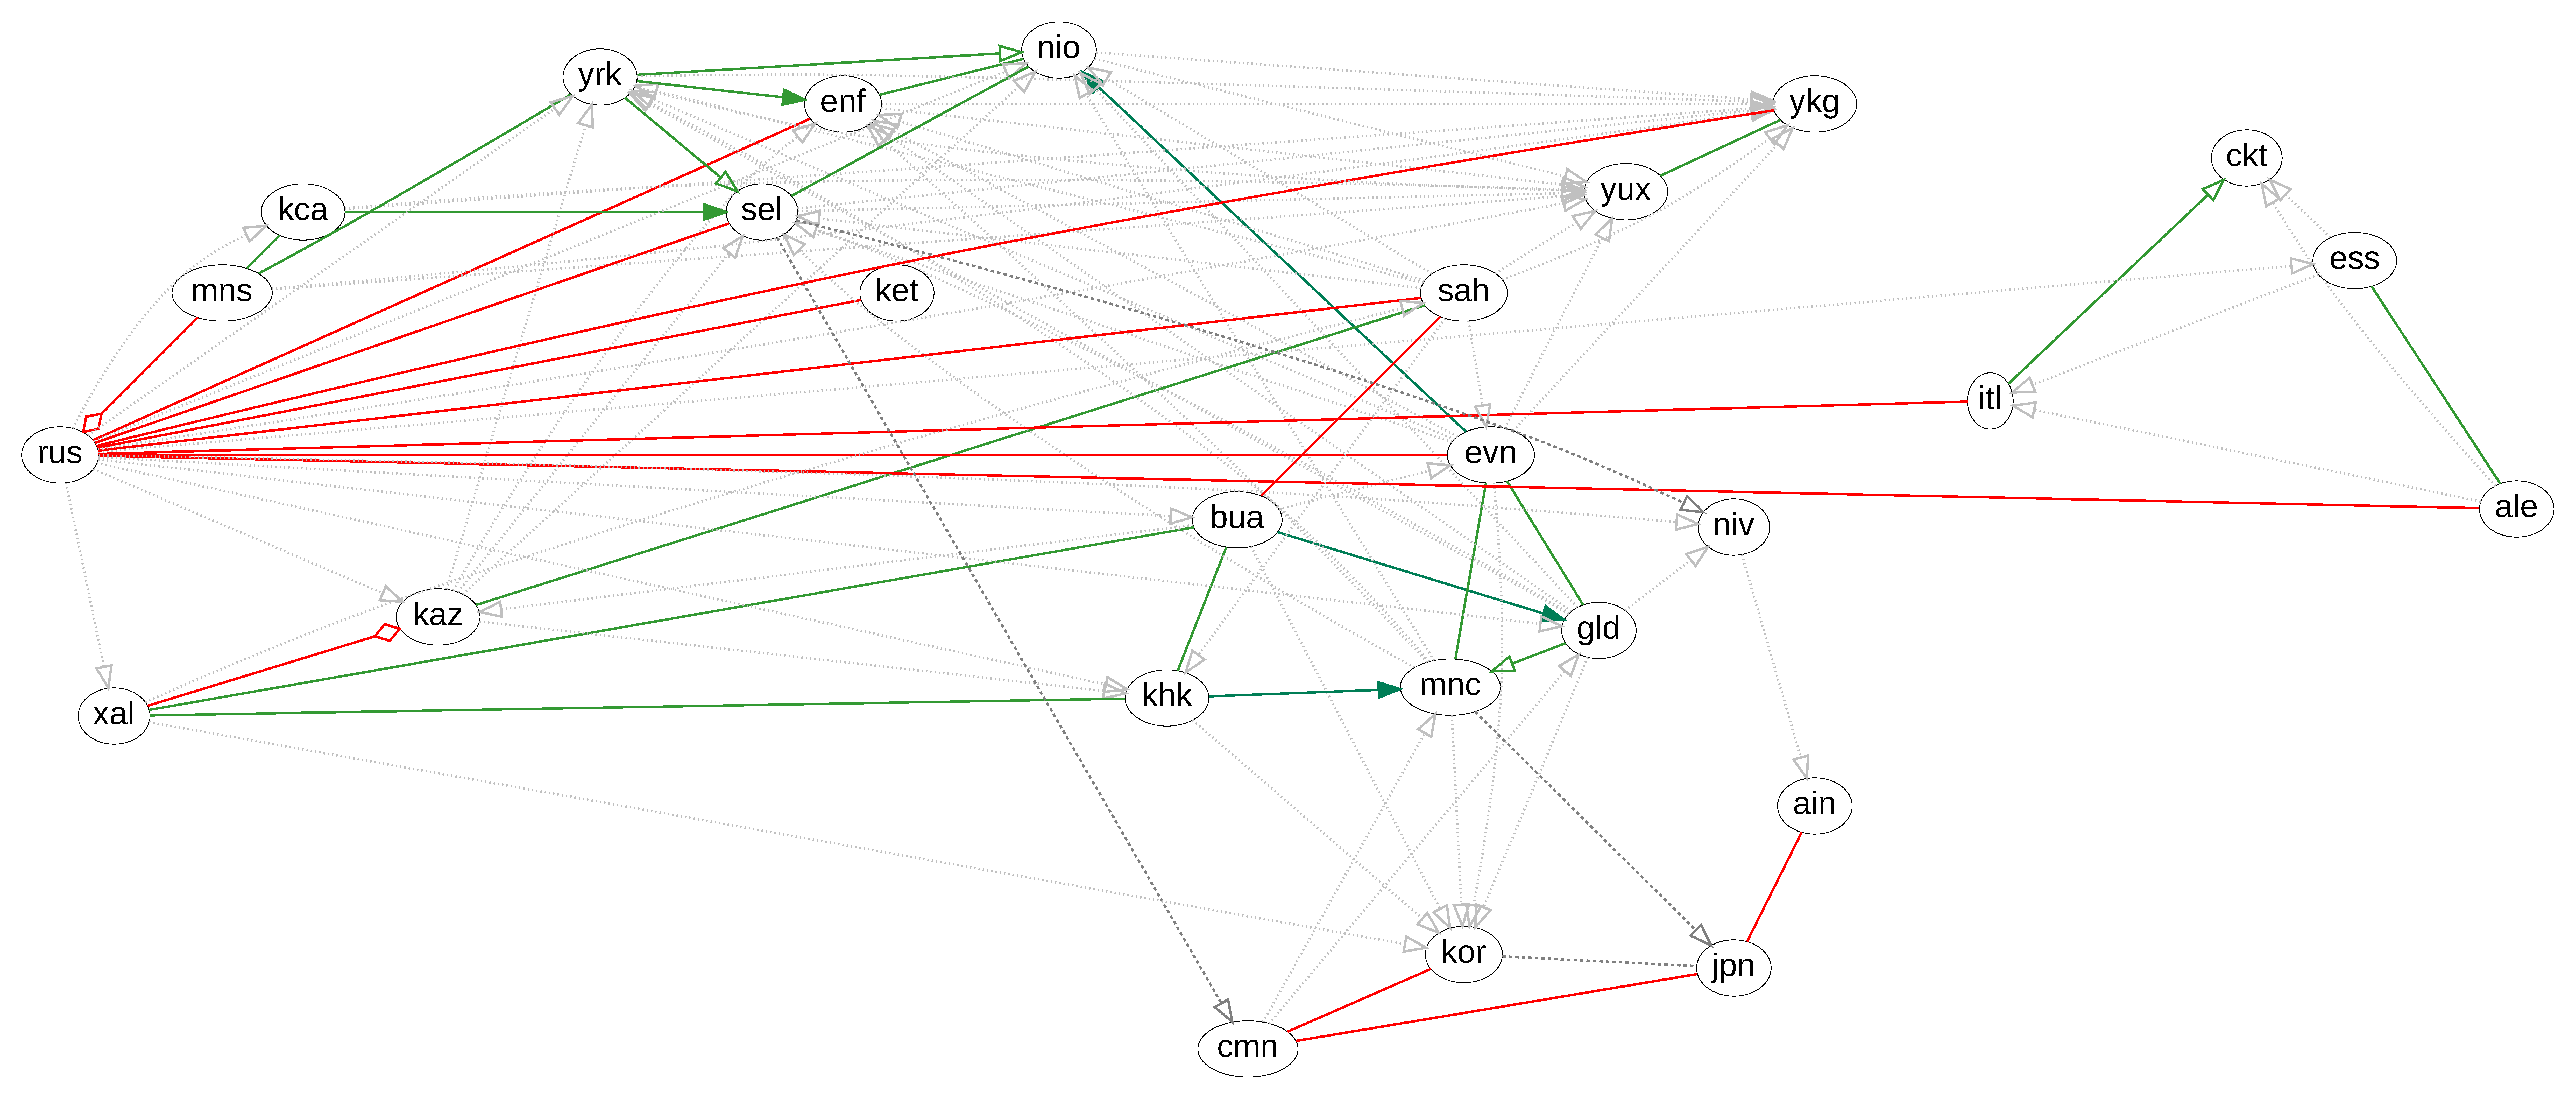
\includegraphics[width=\textwidth]{figures/siberia-contact-fs-tss-eval.pdf}
 \caption{Result and evaluation of contact flow on Siberian data.}
 \label{siberia-result-contact}
\end{figure}
 
 In this scenario, the results of CLFI are actually worse than those of PLFI. As the results in Figure \ref{siberia-result-contact} show, the star-shaped influence of \ili{Russian} on various minority languages is not recognized any more, in most cases leading to bidrectional arcs. This is again due to a lack of high-overlap triples involving the links in question. In the global NorthEuraLex network, the star pattern was inferred just as intended, because there were other \ili{Slavic languages} in the dataset which could serve to form high-overlap triples involving Russian. To see even more clearly how this problem is ingrained in the mechanics of TSS computation, let us take a look at some details behind the pair $rus \arrowLL sah$. The following third languages contribute the most to the triangle score sum: \ili{Kazakh} (30.3\%), \ili{Itelmen} (12\%), \ili{Buryat} and \ili{Kalmyk} (at 6.7\% each). We only have $|cog(rus,sah,kaz)| = 7$, against an overlap of 3.74 predicted for $rus \arrowLA sah \arrowAL 
kaz$, and 13.36 for $sah \arrowLA rus \arrowAL kaz$. The fit of both predictions with the true overlap is thus about equal. This pattern repeats for the other triangles, so that the score ratio reaches only 1.029, a signal which is weaker than any reasonable threshold. For other minority languages, the pattern repeats itself, even if some pairs like $rus \arrowLA ykg$ (TSS ratio 1.357) are much closer to the threshold. So why did everything work much better on the larger scenarios? The reason is that any additional Slavic language such as \ili{Ukrainian} will provide a high-overlap unshielded triple $ukr \arrowLL rus \arrowLL sah$, because Russian will screen off the Russian minority languages from $ukr$ during skeleton inference. The TSS criterion yields very high evidence against this being a v-structure, which tips the balance in favor of arrows going out of Russian for all languages Russian separates from Ukrainian. To summarize, TSS helps to aggregate and weight evidence from different triples, but in 
the absence of unshielded triples creating strong directional signals, TSS will be unstable or inconclusive. Using a pairwise score like TSS does not provide a means to overcome the theoretical results about causal inference, which tell us that unshielded triples are needed to securely establish the direction of causality.
 
 A further interesting phenomenon is displayed by the two-member Chukotko-Kamchatkan\il{Chukotko-Kamchatkan languages} family. \ili{Itelmen} ($itl$), the language whose lexicon was influenced much more strongly by Russian, is inferred to have been the intermediary for transmitting the Russian loans into \ili{Chukchi} ($ckt$), yielding a directional signal between the two related languages. This is a problem that is especially virulent in small language families, which is why we have not yet seen it in the other case studies. The wrong internal structure of Tungusic\il{Tungusic languages} is also created by $evn$ as the obvious entry point for all the Russian loans, which then get transmitted within the family on the path $evn \arrowLA gld \arrowLA mnc$, although this effect is not strong enough to yield a directional signal above the threshold.
 
 Finally, failure to recognize the directionality of contacts between \ili{Chinese}, \ili{Japanese}, and \ili{Korean} is again due to the absence of high-overlap triples that would yield directional information. The most relevant triple for all connections between these three isolates (in our study) is the one formed by the three languages. But the three-way overlap between the three languages is only very small at $|cog(cmn,jpn,kor)| = 14$, showing that the expected problems with recognizing Chinese loans based on \ili{Mandarin Chinese} have indeed materialized. In this triangle, there is not enough room for different directions to vastly differ in the fit of their prediction to the true overlap size, leading to hints of equal strength in every direction. In general, lexical flow inference will always run into problems when isolates are involved, and we can only expect it to work well if both languages connected by the link of interest have close relatives in the dataset. This is the reason why contact flow inference worked so much better on the Baltic Sea and Uralic testsets (where larger families meet) than in isolate-ridden Siberia, where even the colonial language is an isolate in our dataset.
 
 \subsubsection{Case study 4: a visit to the Caucasus}
 \begin{figure}[h!]
 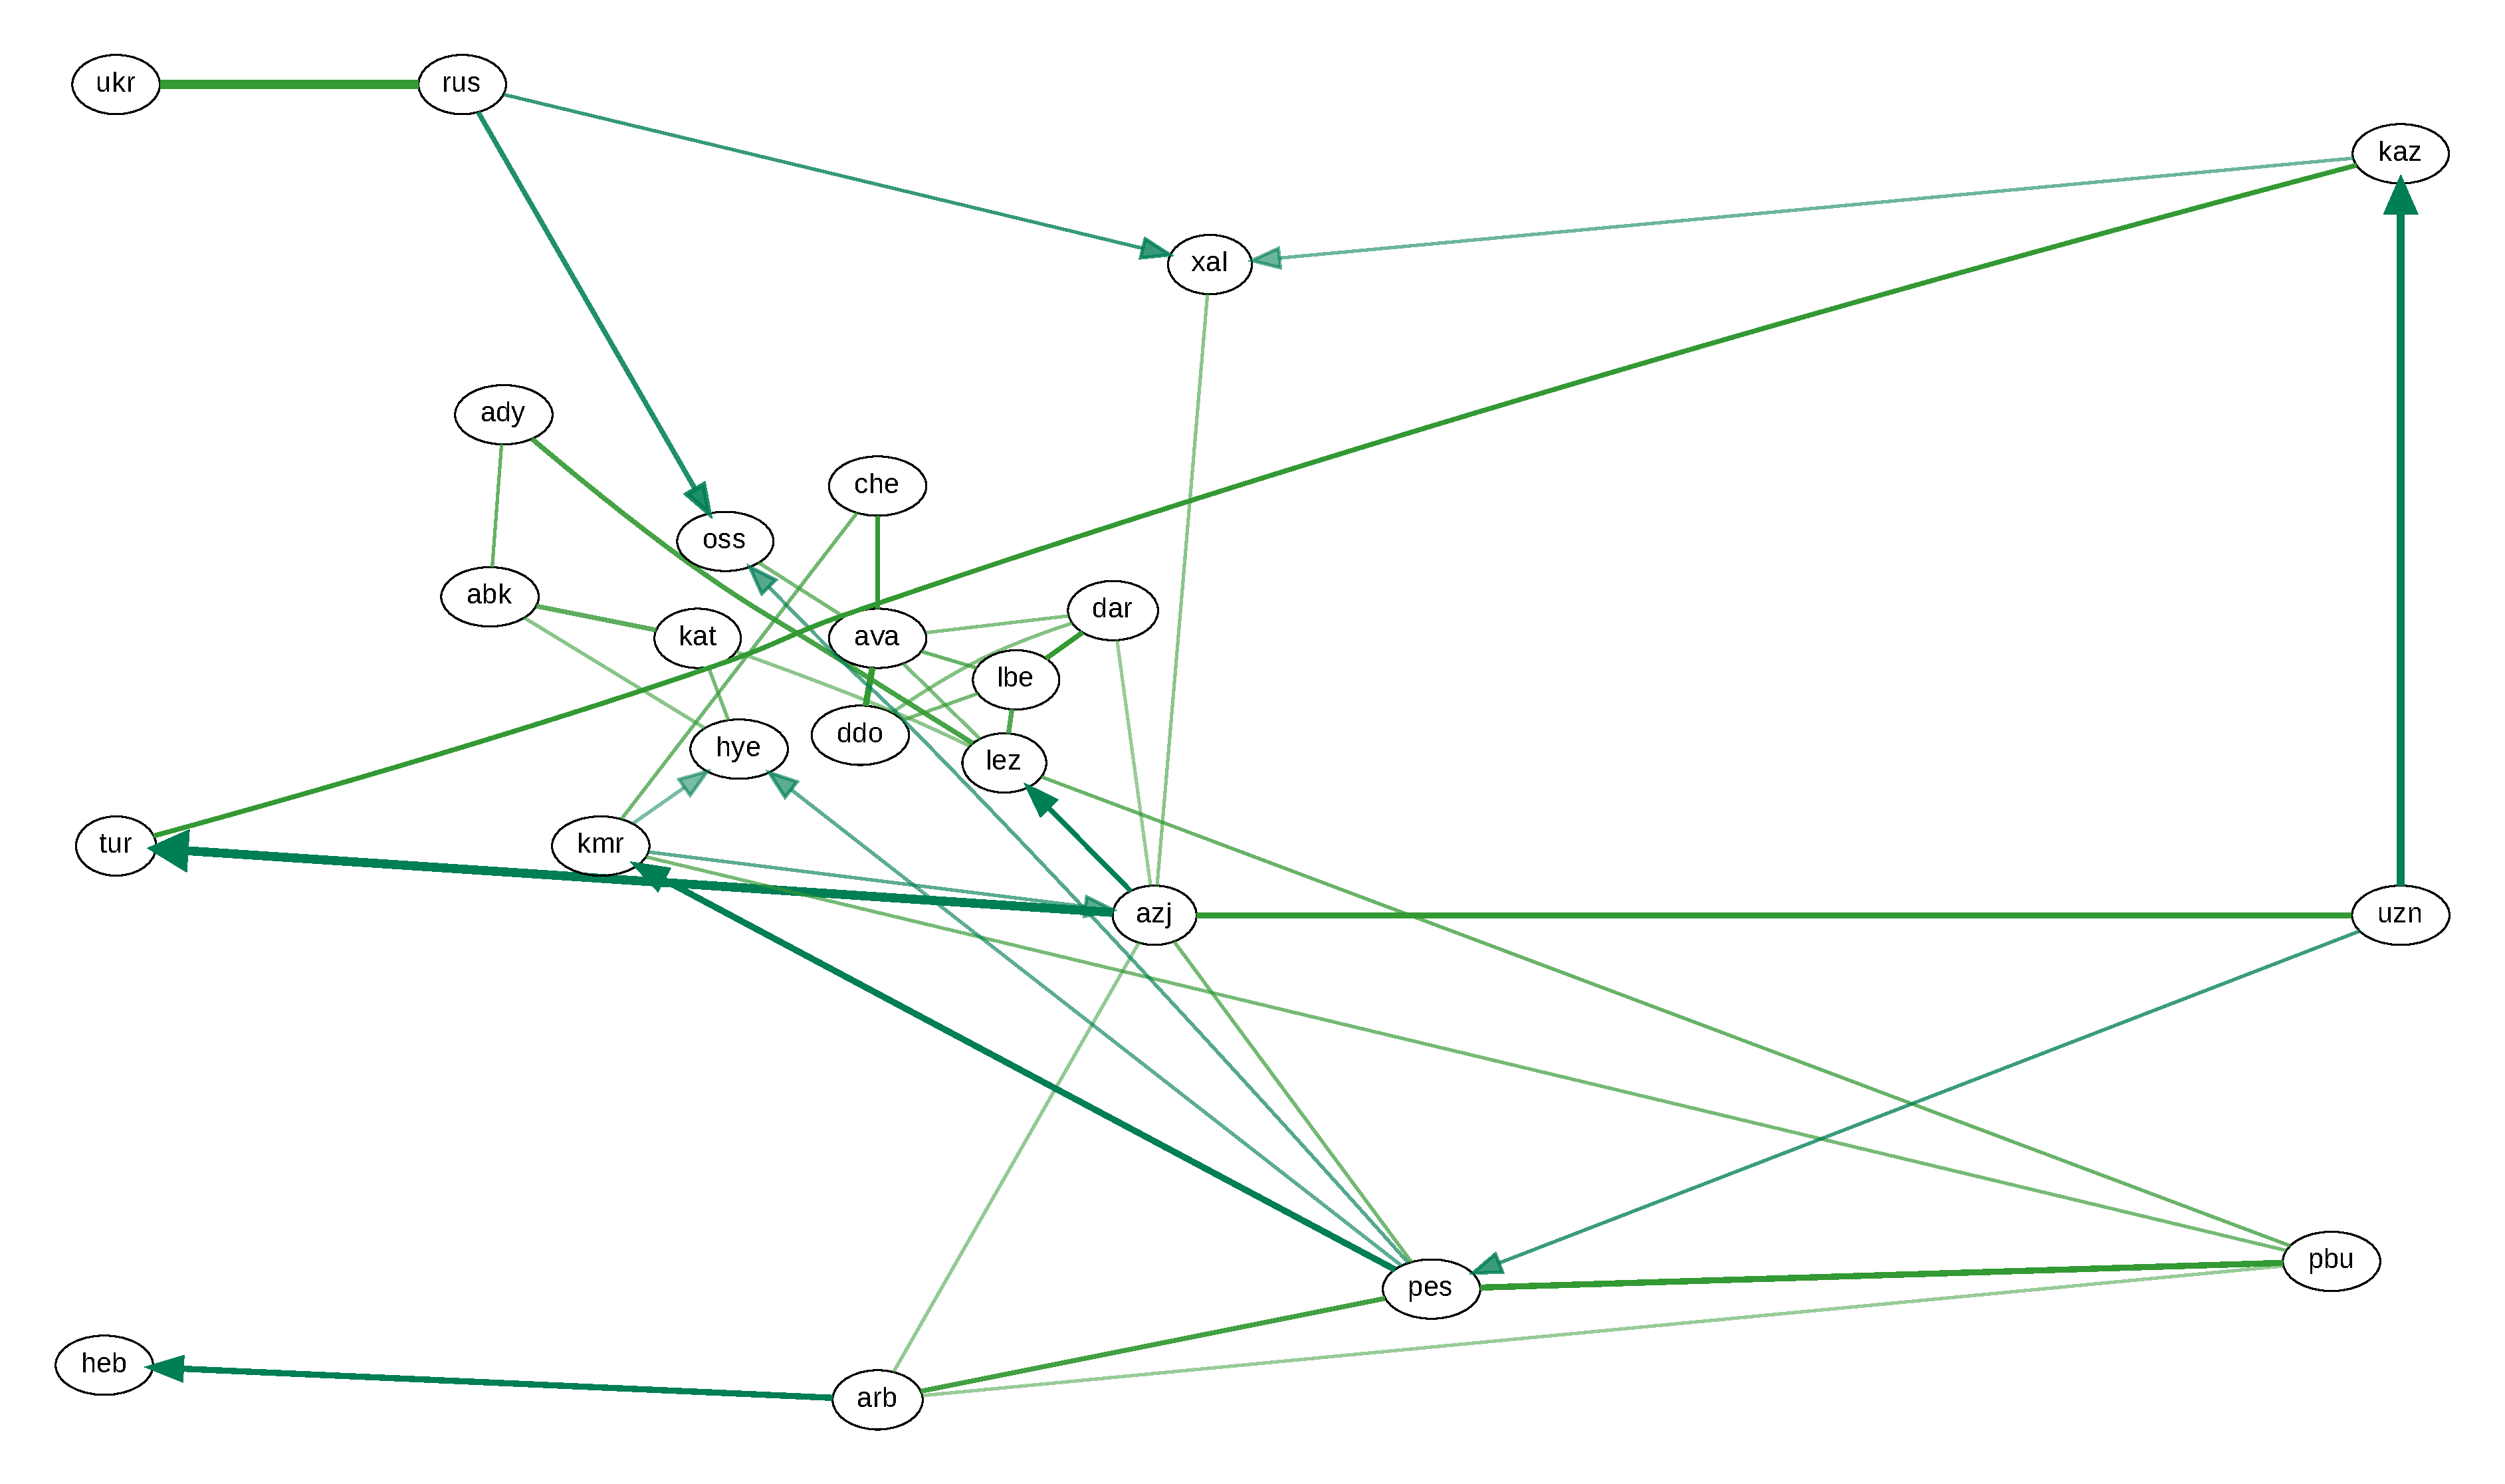
\includegraphics[width=\textwidth]{figures/caucasus-contact-fs-tss.pdf}
 \vspace*{5mm}
 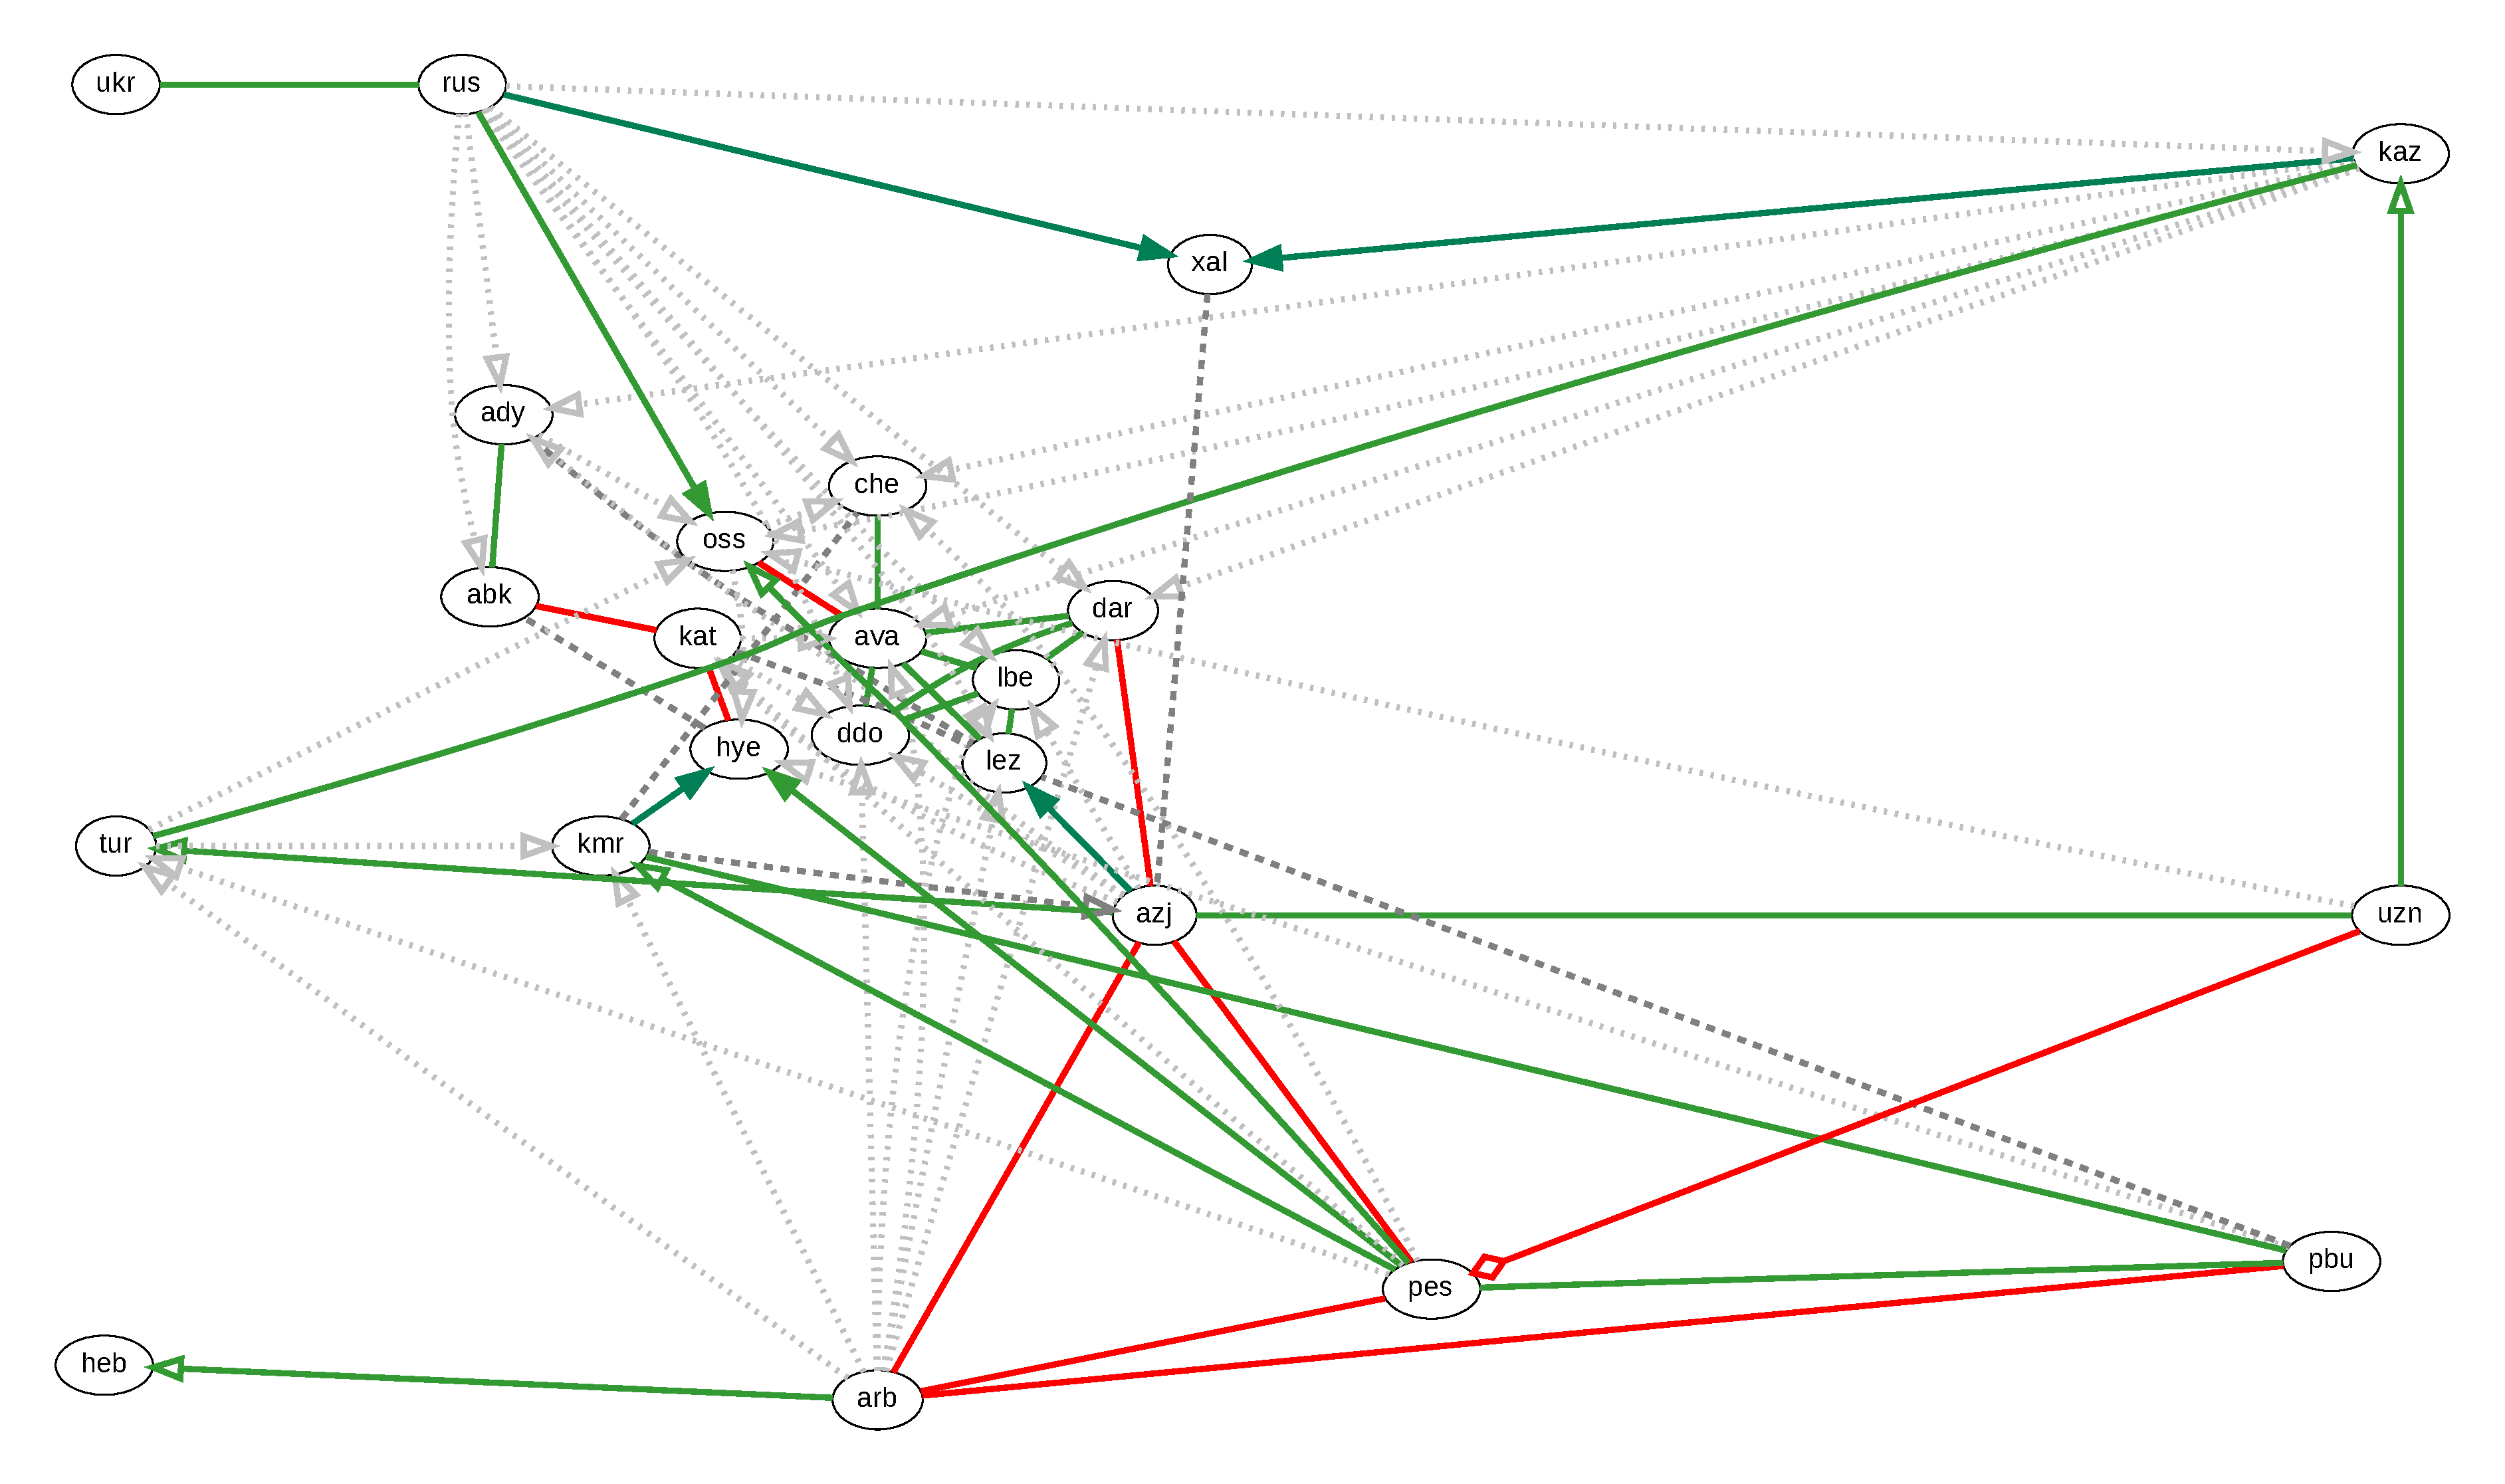
\includegraphics[width=\textwidth]{figures/caucasus-contact-fs-tss-eval.pdf}
 \caption{Result and evaluation of contact flow on Caucasian data.}
 \label{caucasus-result-contact}
 \end{figure}
 
 In the results on the Caucasian case study visualized in Figure \ref{caucasus-result-contact}, it turns out that the absence of a proto-language does not help us to prevent the erroneous arrow from \ili{Uzbek} into \ili{Persian}. The reason is that all the triangles formed from two Turkic languages plus Persian look very much like v-structures according to the predicted overlaps. This is not an issue of data sparseness as in previous cases, because the three-way overlap for such triples will typically exceed 60 cognates. Instead, the problem now is the very high overlap between the \ili{Turkic languages}, which would lead to a three-way overlap of the predicted size even if the true story were a v-structure. This is an instance of one of the cases where the TSS criterion is inadequate.
 
 The second interesting question in this case study is why \ili{Arabic}, which was correctly established to be a major external source of lexical material for the region in UFR-based PLFI, is a source of problems for TSS-based CLFI. Again looking at the TSS score ratios first, we find that the main problem is the triple of \ili{Persian}, Arabic, and \ili{Pashto}, with an overlap of $|cog(arb,pes,pbu)| = 70$ which does not fit the story $arb \arrowLA pbu \arrowLA pes$. The problem here is the assumption of independent sampling. The Arabic loans in Persian and Pashto overlap a lot more than the assumption of independent contacts would suggest, because they are concentrated in the religious and scientific vocabulary. This non-collider signal counteracts the collider signals coming from triples such as $arb \arrowLL pes \arrowLL kmr$. To alleviate this type of problem, one would need a much more explicit flow model which would model the flow beyond the local configuration, enforcing the constraint that there must be a directed path between any pair of languages that share a syubstantial marker of cognates, and takes this into consideration when making local directionality decisions. Unfortunately, it is highly unlikely that inference such a flow model would be tractable at the scale at which I am operating.

\subsection{Evaluation on simulated data}
As the final part of this chapter, I again check whether we can reproduce our findings about the relative performance of different CLFI variants on the simulated data. This time, a little more thought than before must go into the definition of the gold standard. 

\subsubsection{True and detectable histories}
For NorthEuraLex, the inclusion of a contact link into the gold standard presupposed the existence of a discernable layer of loans in the attested part of the language. While this was sometimes difficult to assess based on the available literature, it still provided an external way of getting at the desired information, and the resulting evolutionary network was already relatively flat similar to a contact flow network, because ancient contacts are less clearly known, and less frequently discussed in general descriptions of individual languages.

The main issue in generating such gold standard graphs for the simulated scenarios can be conceptualized as the difference between true and detectable histories. The \textit{true history} is what actually happened during the simulation (including contacts with substrate languages, i.e.\ languages without living descendants about whose existence we can only new due to loanwords they left in attested languages), and is easy to define based on the simulation trace.

In contrast, the \textit{detectable history} is only a subset of the events contained in the true history, informally defined as containing all the events of which some trace is still visible in the cognate data for living languages. By means of the detailed protocol of the complete history for each simulated scenario, the visibility of each event can be determined exactly by checking whether it is part of any word trace leading to a cognacy relation in the input data.

\subsubsection{Summarizing generated contact histories}
A true history gold standard will simply contain every contact link through which more than 25 lexical items were transmitted (based on 1,000 simulated concepts, and our CMI threshold of 0.025). However, expecting CLFI to infer this true history will not lead to a fair assessment of the system's performance. Instead, we need a gold standard that is comparable in difficulty to the equivalent task on the NorthEuraLex data. In other words, we need a way to extract a picture of the history of the linguistic region from the simulation protocols that is roughly comparable in shape and abstraction level to the NorthEuraLex gold standard.

This leads me to the following solution for generating gold standard graphs for the simulated data: Exploiting the existing infrastructure for tracing the history of every attested word (the detectable history), we consider each pair of languages in turn, and count the number of current words that were once borrowed from one language or one of its ancestors to the other language or one of its ancestors, stopping once we meet the lowest common ancestor of both languages. After discarding borrowing events which took place within the same cognate class, we arrive at a total number of transferred items in both directions, and put the appropriate arrow into the gold standard network if the number of borrowings in the respective direction exceeds 10 lexical items.

\subsubsection{Results}
Again, we start with the skeleton performance data in Table \ref{contact-skeleton-evaluation-simulated}. The skeleton recall numbers are globally much better than on the NorthEuraLex data, and the differences between the different separation methods, and especially the difference between PC and FCI skeletons, are again rather small. Since the simulated gold standards based on detectable histories are defined in a much more objective way than the NorthEuraLex gold standard, the difference in recall suggests that a large portion of the contacts postulated by the NorthEuraLex data might not actually be detectable from the data, and that quite a few links, especially those reflecting very ancient contacts, should be removed from the gold standard. Apart from this difference, the small divergences in performance between skeleton inference methods show a very similar pattern as on the NorthEuraLex data, although this time, FCI consistently performs better than the vanilla PC algorithm. This difference once more illustrates that FCI can only play out its strengths on very clean datasets such as my simulated data, whereas it appears very prone to the type of noise seen in automatically inferred cognacy overlap data.

\begin{table}[h]
 \centering
 \begin{tabular}{ccccc}
 \hline \hline
   & \multicolumn{2}{l}{Overlap separation} & \multicolumn{2}{l}{Flow separation}\\ 
   & VPC & FCI & VPC & FCI\\ 
 \hline
  skPrc & \textbf{0.966} & 0.963 & 0.933 & 0.934\\
  skRec & 0.559 & 0.621 & 0.740 & \textbf{0.750}\\
  skFsc & 0.708 & 0.755 & 0.825 & \textbf{0.832}\\
  \hline
 \end{tabular}
 \caption{Comparing CLFI skeleton performance on simulated data.}
 \label{contact-skeleton-evaluation-simulated}
\end{table}

The numbers for arrow performance in Table \ref{contact-arrow-evaluation-simulated} show that as in PLFI, the vanilla variant of causal inference fares a lot better on simulated data than on NorthEuraLex, very likely again due to the absence of noise, as opposed to the relatively high level of noise resulting from automated cognate clustering. Also, the FCI and VCI method show some promise on the simulated data, whereas FCI was was almost useless on NorthEuraLex. This is different to our observations when evaluating PLFI on simulated data, where the TSS directionality influence was clearly the best. The reason for this might be that the theory behind TSS was not adapted to the possible presence of hidden common causes. In comparison to PLFI, the arrow F-scores of the best method are a bit worse. The best arrow F-score on the MLmlt reconstruction was reached by the TSS method at 0.447, whereas we are now at 0.407 with the FS-VCI variant.

\begin{table}[h]
 \centering
 \begin{tabular}{cccccc}
  \hline \hline
   & \multicolumn{5}{l}{Overlap separation}\\ 
        &   VPC &   FCI &   VCI &   UFR &   TSS \\ \hline
  arPrc & 0.366 & \textbf{0.529} & 0.366 & 0.405 & 0.434\\
  arRec & 0.486 & 0.452 & 0.486 & 0.409 & \textbf{0.513}\\
  arFsc & 0.417 & \textbf{0.488} & 0.417 & 0.407 & 0.470\\
  \hline
 \end{tabular}\\[0.5cm]
  \begin{tabular}{cccccc}
  \hline \hline
   & \multicolumn{5}{l}{Flow separation}\\ 
        &   VPC &   FCI &   VCI &   UFR &   TSS\\ \hline
  arPrc &  0.272 & 0.283 & \textbf{0.405} & 0.256 & 0.325\\
  arRec & 0.452 & 0.404 & 0.409 & \textbf{0.516} & 0.504\\
  arFsc & 0.339 & 0.332 & \textbf{0.407} & 0.342 & 0.395\\
  \hline
 \end{tabular}
 \caption{Comparing CLFI arrow performance on simulated data.}
 \label{contact-arrow-evaluation-simulated}
\end{table}

Next, Table \ref{contact-variant-comparison-simulated} ranks all the variants of CLFI according to their combined performance score on the simulated data. It is interesting that the performance on NorthEuraLex data is quite consistently much worse then on the simulated data, although as for PLFI, combination of flow separation with the more robust VCI, TSS and UFR methods does not suffer as much from this. Unlike for CLFI, very different methods end up in the top ranks on simulated and NorthEuraLex data, with only the FS-TSS method staying in one of the top positions across data types. This seems to indicate that the way in which the gold standard was extracted from the simulated data might be not the perfect choice.

Though not the best-performing method on the simulated data, FS-TSS is clearly the best method according to the phylum separation measure. Separating the phyla appears not only to work well on selected example scenarios (such as the Baltic and Uralic case studies), but also across 50 sometimes rather challenging simulated scenarios. This shows that FS-TSS might be a useful tool for discerning different language families in situations which at first sight look rather chaotic.

\begin{table}[h]
 \centering
 \begin{tabular}{lrrrrr}
\hline \hline
CLFI Variant & simulated & NELex  & difference & rank on NELex & phyloSep\\ 
\hline
\texttt{OS-FCI} & 0.368 & 0.137 & -0.231 & 6 & 0.714\\
\texttt{OS-TSS} & 0.355 & 0.140 & -0.215 & 5 & 0.737\\
\texttt{FS-TSS} & 0.329 & 0.283 & -0.046 & 1 & 0.783\\
\texttt{OS-VPC} & 0.315 & 0.104 & -0.211 & 7 & 0.711\\
\texttt{OS-VCI} & 0.315 & 0.103 & -0.212 & 8 & 0.711\\
\texttt{FS-VCI} & 0.288 & 0.252 & -0.036 & 2 & 0.738\\
\texttt{OS-UFR} & 0.288 & 0.151 & -0.137 & 4 & 0.738\\
\texttt{FS-FCI} & 0.283 & 0.088 & -0.195 & 9 & 0.642\\
\texttt{FS-UFR} & 0.282 & 0.242 & -0.040 & 3 & 0.723\\
\texttt{FS-VPC} & 0.282 & 0.071 & -0.211 & 10 & 0.673\\
  \hline
 \end{tabular}
 \caption{CLFI variants ranked by combined F-Score on the simulated data.}
 \label{contact-variant-comparison-simulated}
\end{table}

Summing up the results of CLFI, we have seen in the case studies that while the problems previously caused by the reconstruction have disappeared, the reliability of v-structure tests appears to have dropped in comparison with PLFI. This is perhaps not too surprising, as only the phylogenetic lexical flow paradigm has clear instances of the lexicon of one language being in a very literal sense a mixture of words from other languages. In contrast, contact flow is frequently faced with situations where parts of the overlaps in the triple are actually due to common inheritance, leading to much more unpredictable overlap patterns, and hence to lower performance of v-structure tests. Still, the overall quality of CLFI results was quite comparable with PLFI, giving us another tool for data exploration that also performs quite well at phylum separation.
